\documentclass[10pt,doublecolumn]{IEEEtaes}

\usepackage{url}
\usepackage{graphicx}
\usepackage{textcomp}
\usepackage{xcolor}
\usepackage{amsmath,amssymb,amsfonts}
\usepackage{bm}
\usepackage{multirow}
\usepackage{array}
\usepackage{algorithmicx,algorithm,algpseudocode}
\usepackage{subcaption}
\usepackage{hyperref}
\usepackage{tikz}
\usetikzlibrary{arrows.meta,positioning,fit}

\renewcommand{\algorithmicrequire}{\textbf{Input:}}
\renewcommand{\algorithmicensure}{\textbf{Output:}}
\hyphenation{op-tical net-works semi-conduc-tor}

\begin{document}

\title{SGGT-Net: Spectral-Graph Neural Motion Prediction with Causal Group-Innovation Correction for Maneuvering Group Target Tracking}

\author{KAILUN SHEN}
\affil{Xidian University, Xi'an, China}

\author{WEIMING YUAN}
\affil{Xidian University, Xi'an, China}

\authoraddress{Authors' address: Kailun Shen is with the Institute of Information Sensing, Xidian University, Xi'an 710071, China, E-mail: (\href{mailto:klshen@stu.xidian.edu.cn}{klshen@stu.xidian.edu.cn}); Weiming Yuan is with the Institute of Information Sensing, Xidian University, Xi'an 710071, China, E-mail: (\href{mailto:wmyuan@xidian.edu.cn}{wmyuan@xidian.edu.cn}). {\itshape (Corresponding author: Weiming Yuan.)}}

\maketitle

\begin{abstract}
This paper investigates the problem of tracking maneuvering group targets in cluttered environments. In this problem, motion prediction is affected not only by the individual motion history but also by the common motion changes shared by neighboring targets. Moreover, the residual signal used to identify such changes is formed recursively from uncertain data associations. To address these difficulties, a Spectral-Graph Group Tracking Network (SGGT-Net) is proposed. A graph-based temporal encoder and a Neural ordinary differential equation decoder first generate a one-step motion prior. The historical residuals are processed by a smooth temporal spectral filter to extract low-frequency motion mismatch. Based on the resulting predictor, a causal group-innovation corrector separately encodes the target innovation and a leave-one-out peer innovation. The corresponding whitened innovations, normalized innovation magnitude, and covariance descriptors place the individual and peer residual histories on comparable scales. The corrected prior is incorporated into a belief propagation based tracking framework, where marginal association probabilities are retained during the measurement update. Experiments on in-distribution and out-of-distribution datasets show that the proposed correction reduces the prior position root mean square error from 17.965 m to 16.396 m and from 22.987 m to 20.755 m, respectively. The improvements are more evident during motion switches and strong maneuvers. Complete-tracker experiments further demonstrate stable performance under missed detections and clutter.
\end{abstract}

\begin{IEEEkeywords}
group target tracking, maneuvering target, belief propagation, spectral residual, graph neural network, neural ordinary differential equation
\end{IEEEkeywords}

\section{Introduction}

Tracking multiple interacting targets exhibiting coordinated motion is a critical problem in radar surveillance, maritime monitoring, and airspace management. Unlike conventional multi-target tracking scenarios, group targets often exhibit cooperative motion patterns and strong spatial correlations among trajectories. Due to their importance in both civilian and defense applications, group target tracking has attracted increasing attention in recent years.

Compared with conventional multi-target tracking, group target tracking introduces several additional challenges. First, densely distributed targets lead to highly ambiguous measurement-to-track associations, where incorrect associations may significantly degrade tracking accuracy. Second, the relationships among neighboring targets change with their relative positions and motion states. Behaviors such as group merging and splitting make it difficult to describe these interactions using fixed model parameters. Third, coordinated maneuvers may cause similar prediction errors among several targets. Such errors are easily confused with measurement noise or an isolated association error if only the residual of a single target is considered.

To address these challenges, various group target tracking algorithms have been developed by incorporating interaction-based motion models \cite{shen2025adaptive,zhu2024cbmember,su2023variational}. Among classical probabilistic data association techniques, the joint probabilistic data association filter has been widely applied to group tracking scenarios \cite{lin2021improved,zhang2023group,cong2018group}. Random finite set based methods, such as the labeled multi-Bernoulli and generalized labeled multi-Bernoulli filters, provide a rigorous Bayesian framework for group target tracking \cite{liu2018structure,li2023resolvable}. For instance, Wu et al. developed an LMB-based algorithm for tracking multiple resolvable groups \cite{wu2025tracking}. Li et al. incorporated destination information into a leader-follower model and proposed a new LMB filter for group target tracking \cite{li2023labeled}. In addition, belief propagation (BP) based tracking algorithms approximate marginal association probabilities through message passing on factor graphs and are suitable for tracking multiple closely spaced targets \cite{meyer2018message,shen2026joint}. Li et al. proposed a BP-based approach that jointly estimates group structure and detection probability under a virtual leader model assumption \cite{li2024belief}.

Despite these advances, most existing approaches rely on predefined motion models. Their performance is sensitive to group partitioning and motion-model parameters when the targets perform abrupt maneuvers. Although online parameter estimation alleviates this limitation, the selected model class still constrains the predicted motion \cite{shen2026joint}. A common maneuver is also difficult to distinguish from a noisy measurement when only the instantaneous residual of an individual target is considered.

With the rapid development of deep learning techniques, data-driven approaches have recently been introduced into multi-target tracking. Recurrent neural networks are well suited for modeling the sequential evolution of target states, while graph neural networks (GNNs) can describe relationships among multiple agents. Based on these advantages, several learning-based tracking algorithms have been proposed \cite{zhang2024deep}. Shen et al. introduced a residual spectral feature extraction module and developed an LSTM-based tracker for maneuvering single-target scenarios \cite{shen2024mcst}. Yu et al. employed graph neural networks to learn interactions among group targets and proposed a new LMB filter for group target tracking \cite{yu2024enhancing}. Hu et al. adopted a transformer architecture to separately model short-term maneuvers and long-term motion trends \cite{hu2025mff}. Neural ordinary differential equations (Neural ODEs) have also provided an effective means of representing continuous motion dynamics \cite{chen2018neural}.

The above approaches provide useful descriptions of either temporal maneuvers or inter-target relationships. However, the residual used by an online tracker depends on the preceding prior, posterior, and association result. Independently sampled residual windows therefore do not reproduce the residual sequence encountered during recursive tracking. Furthermore, directly aggregating neighboring residuals may transfer an isolated association error to other targets. These observations motivate a causal correction mechanism in which individual and common innovations are represented separately and normalized by their innovation covariance before fusion.

To this end, this paper adopts the BP algorithm for data association and proposes SGGT-Net for one-step group target motion prediction. The main contributions of this paper are summarized as follows:
\begin{enumerate}
\item A spectral-graph neural motion predictor is developed for maneuvering group targets. A streaming graph temporal encoder represents the evolution of neighboring targets, and a Neural ODE decoder generates the basic one-step prior according to the learned motion dynamics.

\item A temporal spectral residual module is introduced to extract slowly varying motion mismatch from recursively formed residual histories. A smooth filter parameterized by three coefficients preserves the phase relationship of the residual signal and suppresses high-frequency measurement disturbances. The filtered feature is fused with the decoder feature by direct concatenation.

\item A causal group-innovation correction mechanism is designed to refine the basic prior. The target innovation and a leave-one-out peer innovation are encoded through separate branches. Raw innovation histories preserve the direction and magnitude of the motion mismatch, while whitened innovations and covariance descriptors provide scale-normalized information for their fusion. Hence, the correction does not require group-structure labels and only uses information available before the predicted time step.

\item SGGT-Net is incorporated into a BP tracking framework. The soft association probabilities are used in both state moment matching and innovation construction. Motion estimation tests, maneuver-event analysis, complete BP tracking, robustness tests, and ablation experiments are conducted to evaluate the prediction and tracking performance.
\end{enumerate}

The remainder of this paper is organized as follows. Section II formulates the group target tracking problem. Section III introduces the BP-based tracking framework. Section IV presents the proposed SGGT-Net motion prediction architecture. Section V describes the experimental setup and performance evaluation. Finally, Section VI concludes the paper.

\section{Problem Formulation}

This section considers a surveillance scenario in which multiple targets are detected by radar in the presence of clutter and missed detections. The objective is to recursively estimate the kinematic states of all existing targets from the received measurements. No target may generate more than one measurement at a sampling instant, and each measurement originates from at most one target.

At the $k$-th time step, the stacked target state is represented as
\begin{equation}
\mathbf{x}_{k}=\left[\left(\mathbf{x}_{k}^{1}\right)^{T},\ldots,\left(\mathbf{x}_{k}^{N_k}\right)^{T}\right]^{T},
\end{equation}
where $N_k$ denotes the number of existing targets. The state of the $i$-th target is consistently defined as
\begin{equation}
\mathbf{x}_{k}^{i}=\left[p_{k,x}^{i},v_{k,x}^{i},p_{k,y}^{i},v_{k,y}^{i}\right]^{T}.
\label{eq:state_definition}
\end{equation}
The received measurement set is $\mathcal{Z}_k=\{\mathbf{z}_{k}^{1},\ldots,\mathbf{z}_{k}^{M_k}\}$, where $M_k$ includes target-originated measurements and clutter.

\subsection{Target Dynamic Model}

The state evolution of each target is expressed by
\begin{equation}
\mathbf{x}_{k}^{i}=f_k\!\left(\mathbf{x}_{k-1}^{i},\mathcal{X}_{k-1}^{i}\right)+\mathbf{w}_{k}^{i},
\label{eq:general_dynamics}
\end{equation}
where $\mathcal{X}_{k-1}^{i}$ denotes the available histories of the target and its neighboring targets. The process noise satisfies $\mathbf{w}_{k}^{i}\sim\mathcal{N}(\mathbf{0},\mathbf{Q}_{k}^{i})$. The transition function $f_k(\cdot)$ is unknown for a maneuvering group target and is approximated by the proposed network. For reference, the constant-velocity transition matrix is
\begin{equation}
\mathbf{F}_{\mathrm{CV}}=
\begin{bmatrix}
1&\tau&0&0\\
0&1&0&0\\
0&0&1&\tau\\
0&0&0&1
\end{bmatrix},
\label{eq:cv_transition}
\end{equation}
where $\tau$ denotes the sampling interval. Each predicted target state is represented by a Gaussian distribution
\begin{equation}
p(\mathbf{x}_{k}^{i}\mid\mathcal{Z}_{1:k-1})=
\mathcal{N}\!\left(\mathbf{x}_{k}^{i};\hat{\mathbf{x}}_{k|k-1}^{i},\mathbf{P}_{k|k-1}^{i}\right).
\end{equation}

\subsection{Radar Measurement Model}

The radar provides range and azimuth measurements. A measurement generated by the $i$-th target is modeled as
\begin{equation}
\mathbf{z}_{k}^{j}=h\!\left(\mathbf{x}_{k}^{i}\right)+\mathbf{v}_{k}^{j},
\label{eq:measurement_eq}
\end{equation}
where
\begin{equation}
h\!\left(\mathbf{x}_{k}^{i}\right)=
\begin{bmatrix}
\sqrt{(p_{k,x}^{i})^{2}+(p_{k,y}^{i})^{2}}\\
\operatorname{atan2}(p_{k,y}^{i},p_{k,x}^{i})
\end{bmatrix}.
\end{equation}
The measurement noise satisfies $\mathbf{v}_{k}^{j}\sim\mathcal{N}(\mathbf{0},\mathbf{R}_{k})$. Clutter measurements are uniformly distributed over the observation region, and their number follows a Poisson distribution with mean $\mu_c$. The corresponding clutter intensity is denoted by $\kappa(\mathbf{z})$.

\subsection{Data Association Representation}

Following the redundant association representation in \cite{williams2010convergence}, the target-oriented variable $m_k^i$ and measurement-oriented variable $n_k^j$ are defined as
\begin{equation}
m_k^i=
\begin{cases}
j, & \text{target }i\text{ is associated with measurement }j,\\
0, & \text{target }i\text{ is not detected},
\end{cases}
\end{equation}
and
\begin{equation}
n_k^j=
\begin{cases}
i, & \text{measurement }j\text{ originates from target }i,\\
0, & \text{measurement }j\text{ is clutter}.
\end{cases}
\end{equation}
The one-to-one association constraint requires $m_k^i=j$ if and only if $n_k^j=i$. The vector forms are denoted by $\mathbf{m}_k=[m_k^1,\ldots,m_k^{N_k}]^T$ and $\mathbf{n}_k=[n_k^1,\ldots,n_k^{M_k}]^T$.

\section{Factor Graph Based Data Association}

The BP method is employed to calculate marginal association probabilities before the neural state update. This section introduces the factorization and message passing required by the complete tracker. The motion prior in these equations is supplied by SGGT-Net rather than a fixed analytical motion model.

\subsection{Factor Graph Representation}

Let $\psi_i(m_k^i)$ denote the local association evidence of target $i$, and let $\Psi_{ij}(m_k^i,n_k^j)$ enforce the one-to-one constraint. The joint posterior can be factorized as
\begin{equation}
\begin{aligned}
&p(\mathbf{x}_k,\mathbf{m}_k,\mathbf{n}_k\mid\mathcal{Z}_{1:k})\propto\\
&\quad\prod_{i=1}^{N_k}p(\mathbf{x}_k^i\mid\mathcal{Z}_{1:k-1})\psi_i(m_k^i)
\prod_{i=1}^{N_k}\prod_{j=1}^{M_k}\Psi_{ij}(m_k^i,n_k^j).
\end{aligned}
\label{eq:bp_factorization}
\end{equation}
For a detected target, the integrated likelihood ratio is
\begin{equation}
L_{ij}=\frac{P_d^i}{\kappa(\mathbf{z}_k^j)}
\int p(\mathbf{z}_k^j\mid\mathbf{x}_k^i)
p(\mathbf{x}_k^i\mid\mathcal{Z}_{1:k-1})d\mathbf{x}_k^i,
\label{eq:integrated_likelihood}
\end{equation}
whereas the missed-detection evidence is $L_{i0}=1-P_d^i$. The constraint factor is equal to zero for inconsistent assignments and one otherwise. The resulting factor graph is shown in Fig.~\ref{fig:factor_graph}.

\begin{figure}[!t]
\centering
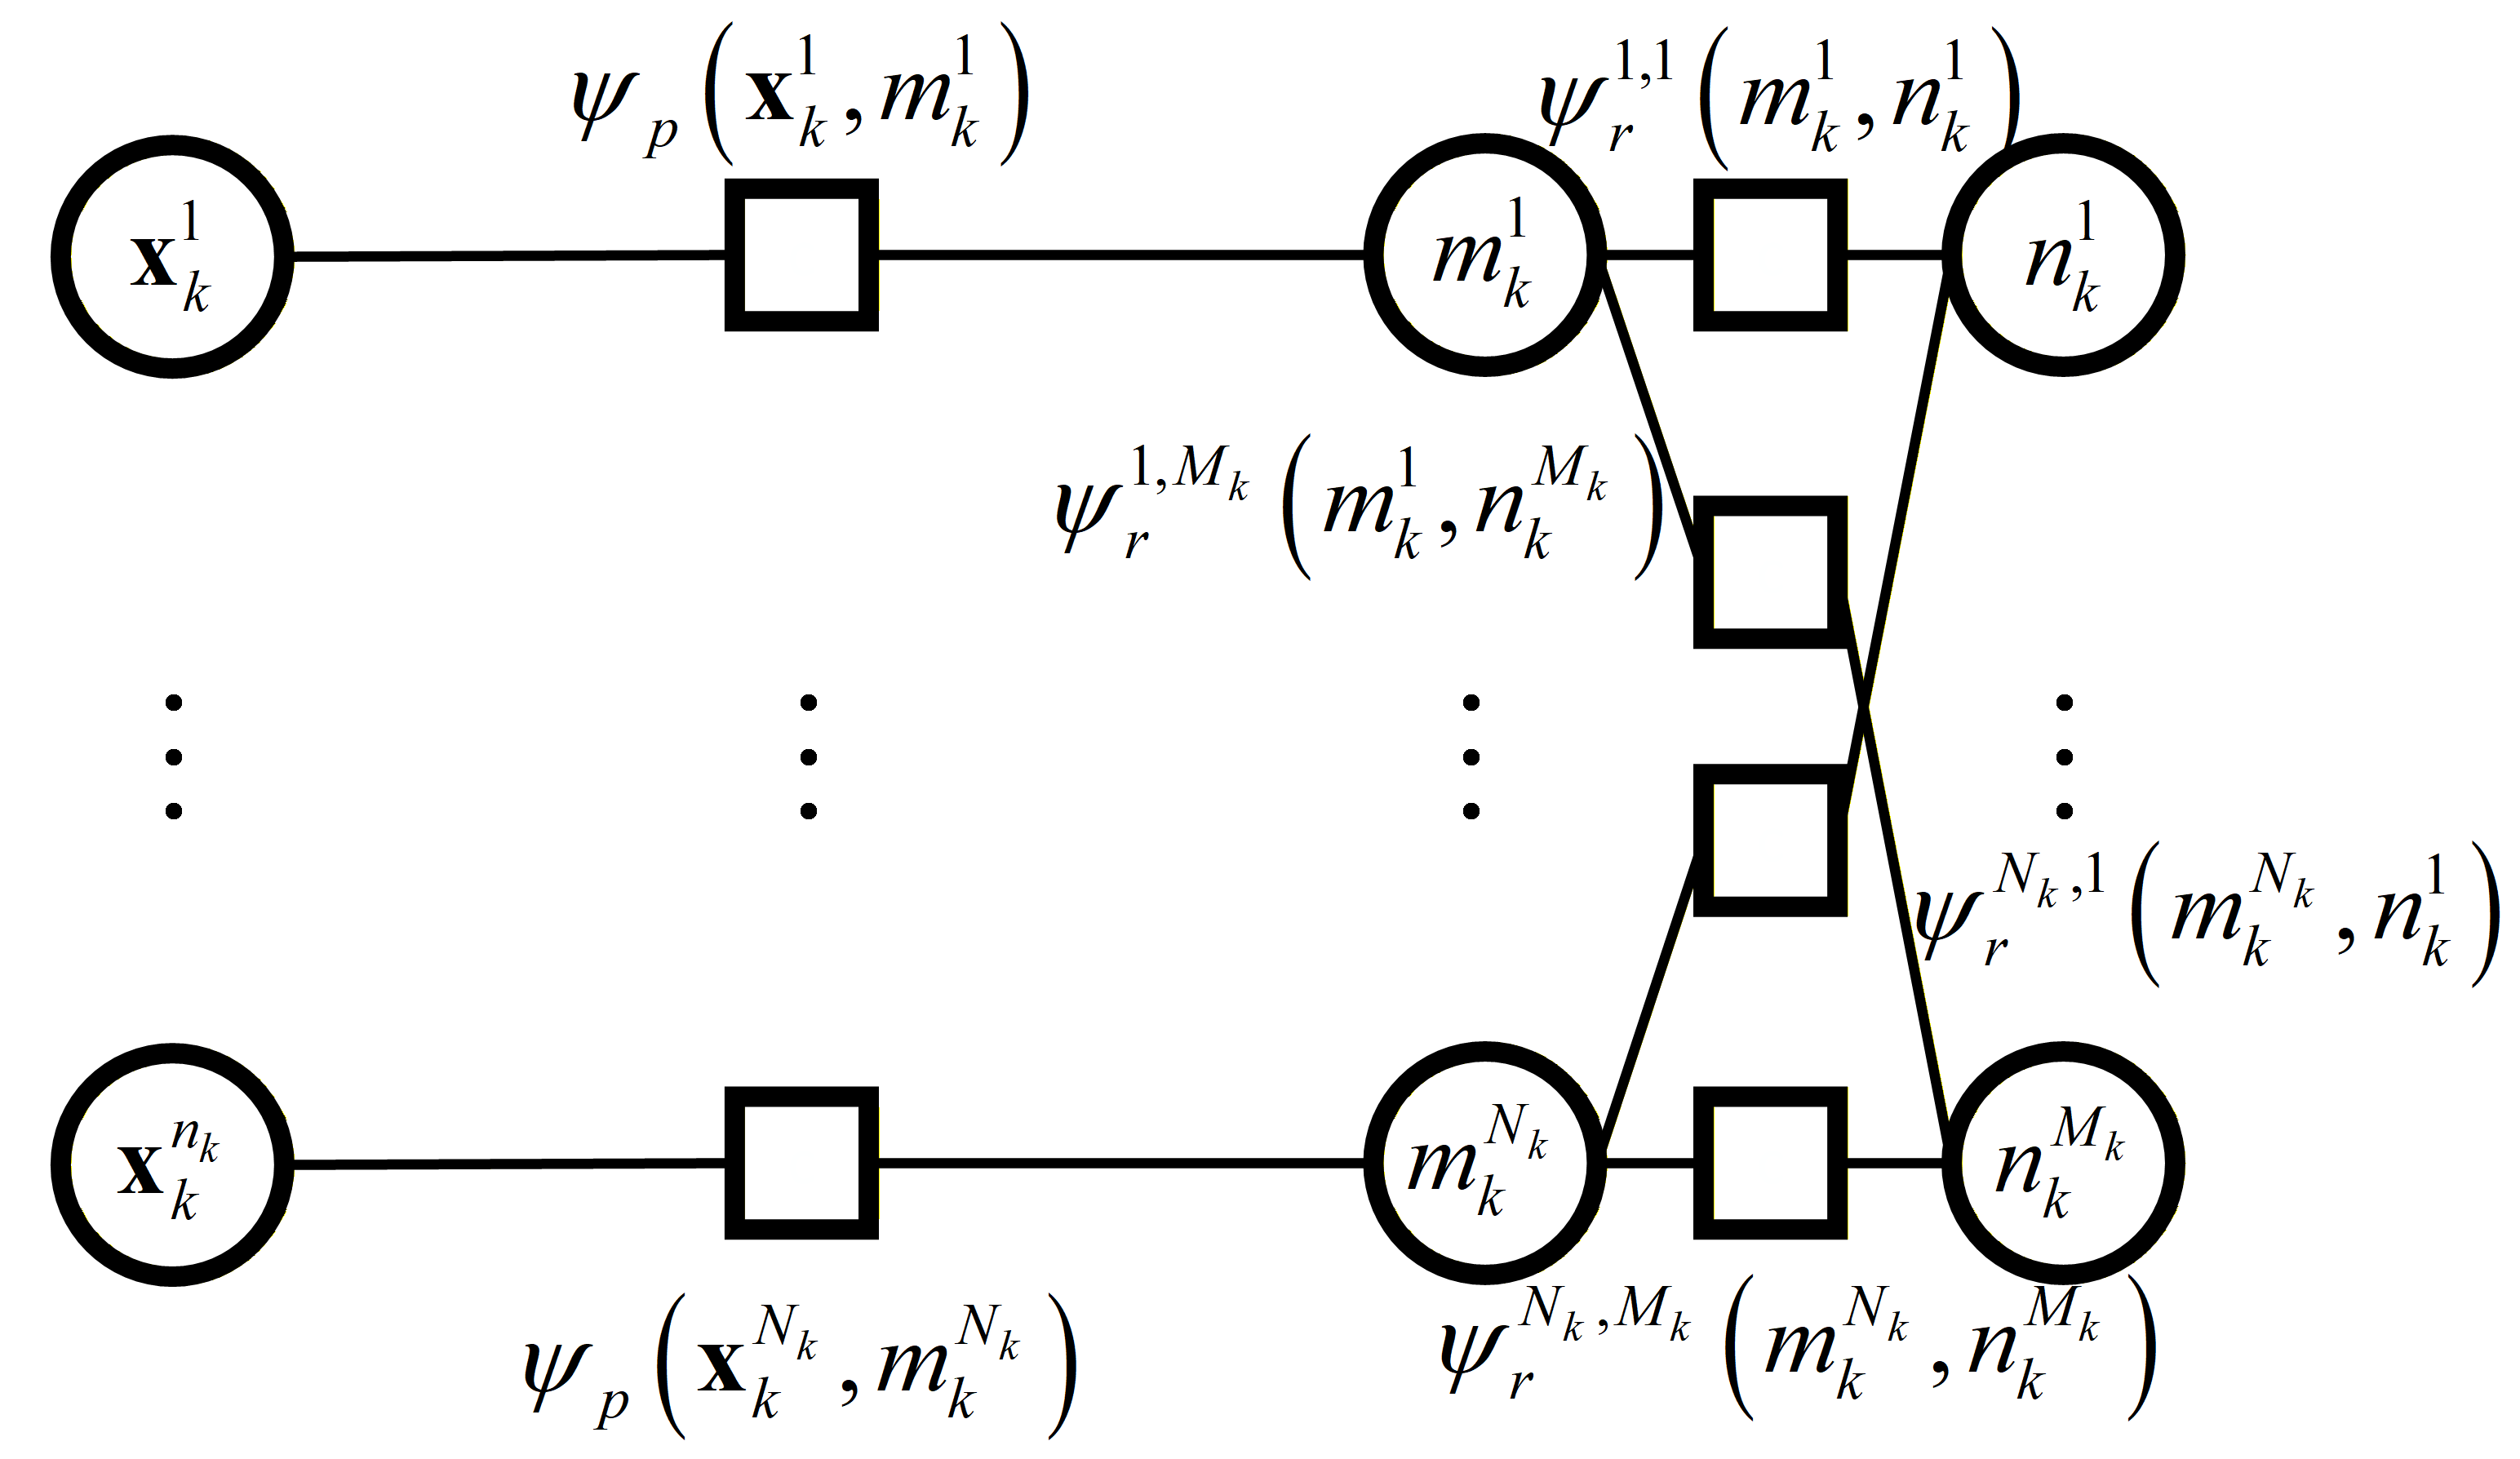
\includegraphics[width=0.72\linewidth]{figures/factor_graph.png}
\caption{Factor graph representation for probabilistic data association.}
\label{fig:factor_graph}
\end{figure}

\subsection{Belief Propagation Message Passing}

The BP messages can be expressed in scalar form. The target-to-measurement and measurement-to-target messages at iteration $q$ are respectively given by \cite{williams2010convergence,meyer2018message}
\begin{align}
\eta_{i\rightarrow j}^{(q)}&=
\frac{L_{ij}}{L_{i0}+\sum_{\ell\neq j}L_{i\ell}\xi_{\ell\rightarrow i}^{(q-1)}},
\label{eq:bp_eta}\\
\xi_{j\rightarrow i}^{(q)}&=
\frac{1}{1+\sum_{r\neq i}\eta_{r\rightarrow j}^{(q)}}.
\label{eq:bp_xi}
\end{align}
The messages are initialized with $\xi_{j\rightarrow i}^{(0)}=1$ and iterated until the prescribed iteration number or convergence tolerance is reached. Only validated target--measurement pairs participate in message passing.

\subsection{Association Probability Estimation}

After message passing, the marginal probabilities of missed detection and target--measurement association are
\begin{align}
\beta_{i0}&=\frac{L_{i0}}{C_i},\\
\beta_{ij}&=\frac{L_{ij}\xi_{j\rightarrow i}}{C_i},\qquad
C_i=L_{i0}+\sum_{j=1}^{M_k}L_{ij}\xi_{j\rightarrow i}.
\label{eq:association_probability}
\end{align}
Thus, $\beta_{i0}+\sum_j\beta_{ij}=1$. These probabilities are retained in the state update and used to construct the soft innovation supplied to the proposed network.

\subsection{State Update and Innovation Construction}

Let $(\hat{\mathbf{x}}_{k|k}^{i,j},\mathbf{P}_{k|k}^{i,j})$ denote the Gaussian update conditioned on assigning measurement $j$ to target $i$. The missed-detection component is defined by $\hat{\mathbf{x}}_{k|k}^{i,0}=\hat{\mathbf{x}}_{k|k-1}^{i}$ and $\mathbf{P}_{k|k}^{i,0}=\mathbf{P}_{k|k-1}^{i}$. Instead of selecting the largest association probability, the posterior moments are matched according to
\begin{align}
\hat{\mathbf{x}}_{k|k}^{i}&=\sum_{j=0}^{M_k}\beta_{ij}\hat{\mathbf{x}}_{k|k}^{i,j},
\label{eq:mixture_mean}\\
\mathbf{P}_{k|k}^{i}&=\sum_{j=0}^{M_k}\beta_{ij}
\left[\mathbf{P}_{k|k}^{i,j}+\mathbf{d}_{ij}\mathbf{d}_{ij}^{T}\right],
\label{eq:mixture_covariance}\\
\mathbf{d}_{ij}&=\hat{\mathbf{x}}_{k|k}^{i,j}-\hat{\mathbf{x}}_{k|k}^{i}.
\end{align}
The second term in Eq.~\eqref{eq:mixture_covariance} retains the spread among association hypotheses.

To construct the soft innovation, define the detected-association mass as $d_k^i=\sum_{j=1}^{M_k}\beta_{ij}$. When $d_k^i>0$, the association probabilities conditioned on detection are
\begin{equation}
\tilde{\beta}_{ij}=\frac{\beta_{ij}}{d_k^i},\qquad j=1,\ldots,M_k.
\label{eq:conditional_association_probability}
\end{equation}
The Cartesian innovation corresponding to measurement $j$ and the soft innovation are respectively defined as
\begin{align}
\mathbf{r}_{k}^{i,j}&=\mathbf{z}_{k,c}^{j}-\mathbf{H}\hat{\mathbf{x}}_{k|k-1}^{i},\\
\mathbf{r}_{k}^{i}&=\sum_{j=1}^{M_k}\tilde{\beta}_{ij}\mathbf{r}_{k}^{i,j}
=\bar{\mathbf{z}}_{k,c}^{i}-\mathbf{H}\hat{\mathbf{x}}_{k|k-1}^{i},
\label{eq:innovation}
\end{align}
where $\bar{\mathbf{z}}_{k,c}^{i}=\sum_j\tilde{\beta}_{ij}\mathbf{z}_{k,c}^{j}$. The observation matrix is
\begin{equation}
\mathbf{H}=\begin{bmatrix}1&0&0&0\\0&0&1&0\end{bmatrix}
\end{equation}
and selects the position components. The innovation covariance corresponding to a single measurement hypothesis is
\begin{equation}
\mathbf{S}_{k}^{i}=\mathbf{H}\mathbf{P}_{k|k-1}^{i}\mathbf{H}^{T}+\mathbf{R}_{k,c}^{i}.
\label{eq:standard_innovation_covariance}
\end{equation}
This covariance is used in the measurement likelihood, the hypothesis-conditioned Kalman gain, and the subsequent normalization of the soft innovation, as in the conventional probabilistic data association filter \cite{barshalom2009probabilistic}. The uncertainty caused by multiple association hypotheses is retained in the posterior covariance through Eq.~\eqref{eq:mixture_covariance}. The scalar $d_k^i$ normalizes the detected hypotheses and determines whether an innovation is available. Specifically, $q_k^i=1$ when the target exists and $d_k^i$ exceeds a small validity threshold; otherwise, $q_k^i=0$, and the corresponding innovation is excluded by the history mask rather than replaced by a synthetic residual.

\section{Graph Neural Network Based Motion Prediction}

\subsection{Overall Encoder--Decoder Architecture}

The overall architecture of SGGT-Net is illustrated in Fig.~\ref{fig:architecture}. At each time step, the posterior states are first processed by a streaming graph temporal encoder. The encoder state is updated once, after which the decoder generates a one-step basic prior. Historical residuals are filtered in the frequency domain and fused into the Neural ODE decoder. Finally, the causal group-innovation corrector refines the basic prior using only innovations formed before the predicted time step. The corrected prior and covariance are passed to the BP module at the next measurement update.

\begin{figure*}[!t]
\centering
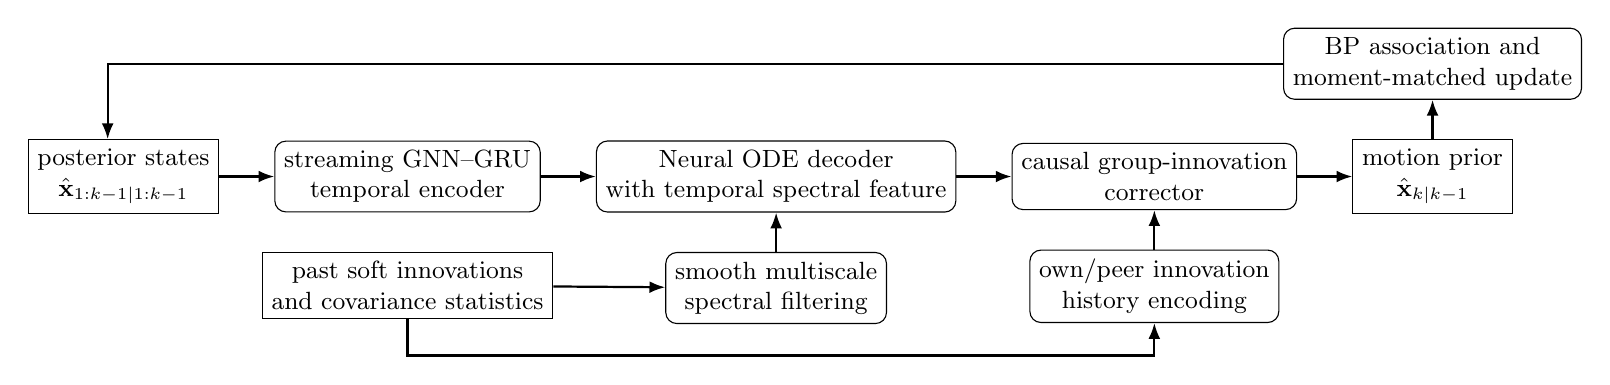
\begin{tikzpicture}[
node distance=5mm and 7mm,
block/.style={draw,rounded corners,align=center,minimum height=8mm,minimum width=21mm,font=\small},
data/.style={draw,align=center,minimum height=8mm,minimum width=20mm,font=\small},
arrow/.style={-{Latex[length=2mm]},thick}
]
\node[data] (post) {posterior states\\$\hat{\mathbf{x}}_{1:k-1|1:k-1}$};
\node[block,right=of post] (enc) {streaming GNN--GRU\\temporal encoder};
\node[block,right=of enc] (ode) {Neural ODE decoder\\with temporal spectral feature};
\node[block,right=of ode] (corr) {causal group-innovation\\corrector};
\node[data,right=of corr] (prior) {motion prior\\$\hat{\mathbf{x}}_{k|k-1}$};
\node[data,below=of enc] (res) {past soft innovations\\and covariance statistics};
\node[block,below=of ode] (fft) {smooth multiscale\\spectral filtering};
\node[block,below=of corr] (peer) {own/peer innovation\\history encoding};
\node[block,above=of prior] (bp) {BP association and\\moment-matched update};
\draw[arrow] (post)--(enc);
\draw[arrow] (enc)--(ode);
\draw[arrow] (ode)--(corr);
\draw[arrow] (corr)--(prior);
\draw[arrow] (res)--(fft);
\draw[arrow] (fft)--(ode);
\draw[arrow] (res.south) |- ([yshift=-4mm]fft.south) -| (peer.south);
\draw[arrow] (peer)--(corr);
\draw[arrow] (prior)--(bp);
\draw[arrow] (bp.west)-|([xshift=-2mm]post.north);
\end{tikzpicture}
\caption{Overall architecture of SGGT-Net within the recursive BP tracking process. All innovation features used to predict time $k$ are formed no later than time $k-1$.}
\label{fig:architecture}
\end{figure*}

\subsection{Graph-Based Temporal Encoder}

An online geometric graph $\mathcal{G}_{k}=(\mathcal{V}_{k},\mathcal{E}_{k})$ is constructed from the current posterior states. Each existing target corresponds to a node, and edges connect spatially neighboring targets within the same scene. The node input contains the normalized position, velocity, and recursively updated hidden state. For an edge $(j,i)$, relative position, relative velocity, distance, and radial motion are used as edge features. These quantities do not require a manually annotated group identity.

Let $\mathbf{h}_{k-1}^{i}$ denote the hidden state of target $i$. A graph message is calculated by
\begin{equation}
\mathbf{m}_{k}^{i}=\sum_{j\in\mathcal{N}_{k}^{i}}\alpha_{ij,k}
\phi_m\!\left(\mathbf{h}_{k-1}^{i},\mathbf{h}_{k-1}^{j},\mathbf{e}_{ij,k}\right),
\label{eq:graph_message}
\end{equation}
where $\phi_m(\cdot)$ is a multilayer perceptron and $\alpha_{ij,k}$ is the normalized graph-attention coefficient. The temporal state is updated by a graph-gated recurrent unit
\begin{equation}
\mathbf{h}_{k}^{i}=\operatorname{GRU}\!\left(\left[\phi_x(\mathbf{x}_{k|k}^{i}),\mathbf{m}_{k}^{i}\right],\mathbf{h}_{k-1}^{i}\right).
\label{eq:graph_gru}
\end{equation}
During a trajectory rollout, Eq.~\eqref{eq:graph_gru} is executed once for each new frame. Hence, the encoder state is propagated forward without repeatedly encoding an overlapping historical window.

\subsection{Temporal Spectral Residual Features}

The innovation sequence contains both motion mismatch and measurement disturbance. The former generally varies continuously over a short interval, whereas the latter is dominated by rapidly varying components. For this reason, the historical residuals are transformed into the frequency domain. For a window of length $L$, the one-sided discrete Fourier transform is
\begin{equation}
\mathbf{R}_{k,L}^{i}(q)=\sum_{\ell=0}^{L-1}\mathbf{r}_{k-L+1+\ell}^{i}
\exp\!\left(-\mathrm{j}\frac{2\pi q\ell}{L}\right),
\label{eq:residual_fft}
\end{equation}
where $q=0,\ldots,\lfloor L/2\rfloor$ is the frequency-bin index. Two residual scales, $L\in\{8,16\}$, are employed. Invalid residual entries are excluded by the corresponding validity mask.

The parameter network first summarizes the spectral distribution.   Let
\begin{equation}
	K_L=\left\lfloor \frac{L}{2}\right\rfloor+1
\end{equation}
denote the number of nonnegative frequency bins. The one-sided
spectrum of the two residual channels is arranged as
\begin{equation}
	\mathbf{R}_{k,L}^{i}
	=
	\left[
	\mathbf{R}_{k,L}^{i}(0),
	\mathbf{R}_{k,L}^{i}(1),
	\ldots,
	\mathbf{R}_{k,L}^{i}(K_L-1)
	\right]
	\in\mathbb{C}^{2\times K_L}.
	\label{eq:complete_residual_spectrum}
\end{equation}
Since the residual sequence is real-valued, this one-sided spectrum
contains all independent Fourier coefficients.

The average spectral energy is first calculated as
\begin{equation}
	E_{k,L}^{i}
	=
	\frac{1}{2K_L}
	\sum_{q=0}^{K_L-1}
	\left\|
	\mathbf{R}_{k,L}^{i}(q)
	\right\|_{2}^{2}.
	\label{eq:residual_spectral_energy}
\end{equation}
Each complex coefficient is then normalized according to
\begin{equation}
	\overline{\mathbf{R}}_{k,L}^{i}(q)
	=
	\frac{
		\mathbf{R}_{k,L}^{i}(q)
	}{
		\sqrt{E_{k,L}^{i}+\varepsilon}
	},
	\qquad q=0,\ldots,K_L-1,
	\label{eq:normalized_residual_spectrum}
\end{equation}
where $\varepsilon$ is a small positive constant introduced for
numerical stability.

The complete spectral descriptor is constructed by concatenating the
real and imaginary parts of all normalized Fourier coefficients with
the logarithmic spectral energy:
\begin{equation}
	\mathbf{s}_{k,L}^{i}
	=
	\begin{bmatrix}
		\operatorname{vec}
		\left(
		\operatorname{Re}
		\overline{\mathbf{R}}_{k,L}^{i}
		\right)
		\\[1mm]
		\operatorname{vec}
		\left(
		\operatorname{Im}
		\overline{\mathbf{R}}_{k,L}^{i}
		\right)
		\\[1mm]
		\log\left(E_{k,L}^{i}+\varepsilon\right)
	\end{bmatrix}
	\in\mathbb{R}^{4K_L+1},
	\label{eq:complete_spectral_descriptor}
\end{equation}
where $\operatorname{vec}(\cdot)$ stacks the coefficients of the two
residual channels over all nonnegative frequency bins. 

A scale-specific two-layer MLP maps the complete spectral descriptor
to three unconstrained filter parameters:
\begin{equation}
	\begin{bmatrix}
		\hat a_{k,L}^{i}\\
		\hat b_{k,L}^{i}\\
		\hat c_{k,L}^{i}
	\end{bmatrix}
	=
	\phi_L
	\left(
	\mathbf{s}_{k,L}^{i};
	\boldsymbol{\theta}_L
	\right),
	\label{eq:abc_parameter_network}
\end{equation}
where $\phi_L(\cdot;\boldsymbol{\theta}_L)$ denotes the parameter
network associated with scale $L$, and
$\boldsymbol{\theta}_L$ contains its learnable parameters.

The constrained filter parameters are defined as
\begin{equation}
	\begin{aligned}
		a_{k,L}^{i}
		&=-\operatorname{softplus}
		\left(\hat a_{k,L}^{i}\right),\\
		b_{k,L}^{i}
		&=-\operatorname{softplus}
		\left(\hat b_{k,L}^{i}\right),\\
		c_{k,L}^{i}
		&=\hat c_{k,L}^{i}.
	\end{aligned}
	\label{eq:abc_parameter_constraints}
\end{equation}
Instead of predicting an independent gain for every frequency bin,
these three parameters generate a smooth frequency response. With the
normalized frequency
$f_q=q/(K_L-1)\in[0,1]$, the response is
\begin{equation}
	g_{k,L}^{i}(f_q)
	=
	\frac{
		\sigma\left(
		a_{k,L}^{i}f_q^2+
		b_{k,L}^{i}f_q+
		c_{k,L}^{i}
		\right)
	}{
		\sigma\left(c_{k,L}^{i}\right)
	}.
	\label{eq:abc_filter}
\end{equation}
Since $a_{k,L}^{i}<0$ and $b_{k,L}^{i}<0$, the derivative of the
quadratic logit satisfies
\begin{equation}
	2a_{k,L}^{i}f_q+b_{k,L}^{i}\leq 0,
	\qquad f_q\geq0.
\end{equation}
Consequently, Eq.~\eqref{eq:abc_filter} produces a nonincreasing
low-pass response, while
$g_{k,L}^{i}(0)=1$ preserves the zero-frequency component.
 
The filtered residual sequence is obtained by
\begin{equation}
	\tilde{\mathbf{r}}_{k,L}^{i}
	=
	\mathcal{F}^{-1}
	\left(
	\left\{
	g_{k,L}^{i}(f_q)
	\mathbf{R}_{k,L}^{i}(q)
	\right\}_{q=0}^{K_L-1}
	\right).
	\label{eq:filtered_residual_sequence}
\end{equation}
Thus,
$\tilde{\mathbf{r}}_{k,L}^{i}\in\mathbb{R}^{L\times2}$
is the filtered time-domain residual sequence. It is mapped to a
scale-specific latent vector by
\begin{equation}
	\boldsymbol{\eta}_{k,L}^{i}
	=
	\psi_L
	\left(
	\tilde{\mathbf{r}}_{k,L}^{i};
	\boldsymbol{\vartheta}_L
	\right)
	\in\mathbb{R}^{d_h},
	\label{eq:scale_temporal_latent}
\end{equation}
where $\psi_L(\cdot;\boldsymbol{\vartheta}_L)$ consists of two
one-dimensional convolutional layers with a SiLU activation between
them, followed by temporal average pooling.
The symbol $\boldsymbol{\vartheta}_L$ contains the learnable convolution parameters, and $d_h$ is the decoder feature dimension. Consequently, $\boldsymbol{\eta}_{k,L}^{i}$ summarizes the filtered residual sequence at scale $L$.

Let $L_{\max}=16$ and let $v_{k,\ell,d}^{i}\in\{0,1\}$ indicate whether residual channel $d\in\{x,y\}$ at position $\ell$ of the complete residual buffer is valid. The valid-history ratio is
\begin{equation}
\gamma_{k}^{i}=\frac{1}{2L_{\max}}
\sum_{\ell=0}^{L_{\max}-1}\sum_{d\in\{x,y\}}v_{k,\ell,d}^{i}.
\label{eq:residual_valid_ratio}
\end{equation}
Each scale is assigned a scalar score
\begin{equation}
e_{k,L}^{i}=\chi_L\!\left(
[\boldsymbol{\eta}_{k,L}^{i},\gamma_{k}^{i}];\boldsymbol{\zeta}_L
\right),
\label{eq:scale_score}
\end{equation}
where $\chi_L(\cdot;\boldsymbol{\zeta}_L)$ is a learnable affine scorer with parameters $\boldsymbol{\zeta}_L$. The normalized scale weights are
\begin{equation}
\omega_{k,L}^{i}=\frac{\exp(e_{k,L}^{i})}
{\sum_{L'\in\{8,16\}}\exp(e_{k,L'}^{i})},
\qquad \sum_{L\in\{8,16\}}\omega_{k,L}^{i}=1.
\label{eq:scale_weight}
\end{equation}
The multiscale spectral feature is finally obtained as
\begin{equation}
\mathbf{s}_{k}^{i}=\phi_{\mathrm{out}}\!\left(
\sum_{L\in\{8,16\}}\omega_{k,L}^{i}\boldsymbol{\eta}_{k,L}^{i}
\right)\in\mathbb{R}^{d_h},
\label{eq:multiscale_spectral_feature}
\end{equation}
where $\phi_{\mathrm{out}}(\cdot)$ consists of a linear projection, layer normalization, and a SiLU activation. In the formal model, this module performs temporal filtering only; graph information enters through the encoder and the group-innovation corrector. The feature $\mathbf{s}_{k}^{i}$ is then concatenated with the graph temporal decoder feature $\mathbf{h}_{k}^{i}$ and projected as
\begin{equation}
\bar{\mathbf{h}}_{k}^{i}=\mathbf{h}_{k}^{i}+
\phi_s\!\left([\mathbf{h}_{k}^{i},\mathbf{s}_{k}^{i}]\right).
\label{eq:concat_fusion}
\end{equation}
Here, $\phi_s(\cdot)$ maps the concatenated $2d_h$-dimensional vector back to $d_h$ dimensions, and $\bar{\mathbf{h}}_{k}^{i}$ is the feature supplied to the Neural ODE motion model.

\subsection{Neural ODE Temporal Predictor}

The temporal predictor maps $\bar{\mathbf{h}}_{k}^{i}$ to the acceleration input of a continuous kinematic model. To simplify the notation, the internal ODE state is arranged as $\mathbf{y}=[p_x,p_y,v_x,v_y]^T$ and is permuted back to the state order in Eq.~\eqref{eq:state_definition} at the output. Its derivative is
\begin{equation}
\frac{d\mathbf{y}^{i}(t)}{dt}=
\begin{bmatrix}
v_x^{i}(t)\\v_y^{i}(t)\\
a_x^{i}(t)\\a_y^{i}(t)
\end{bmatrix},\qquad
[a_x^{i},a_y^{i}]^{T}=\phi_a(\mathbf{y}^{i},\bar{\mathbf{h}}_{k}^{i}).
\label{eq:ode_dynamics}
\end{equation}
The one-step solution is approximated by the fourth-order Runge--Kutta method \cite{kutta1901beitrag}. The resulting state is denoted by $\hat{\mathbf{x}}_{k|k-1}^{i,\mathrm{T}}$ and serves as the temporal basic prior.

\subsection{Causal Group-Innovation Correction}

Although the graph encoder represents the relative motion of neighboring targets, it does not explicitly determine whether a recent prediction error is shared by the neighboring targets. This information is obtained from the innovation history. Based on Eq.~\eqref{eq:standard_innovation_covariance}, the whitened innovation and normalized innovation magnitude are defined as
\begin{align}
\boldsymbol{\nu}_{t}^{i}&=(\mathbf{S}_{t}^{i})^{-1/2}\mathbf{r}_{t}^{i},
\label{eq:white_innovation}\\
\epsilon_{t}^{i}&=(\mathbf{r}_{t}^{i})^{T}(\mathbf{S}_{t}^{i})^{-1}\mathbf{r}_{t}^{i}=\|\boldsymbol{\nu}_{t}^{i}\|_2^2.
\label{eq:association_normalized_innovation}
\end{align}
Whitening places residuals with different predicted covariance on a comparable scale. Since $\mathbf{r}_t^i$ is a probability-weighted soft innovation rather than the innovation of a known measurement hypothesis, $\epsilon_t^i$ is used as a normalized magnitude descriptor and is not assumed to follow an exact chi-square distribution. It reduces to the conventional normalized innovation squared when one measurement hypothesis has probability one.

For target $i$, let $q_t^i\in\{0,1\}$ indicate whether its innovation at frame $t$ is valid, and define the valid leave-one-out neighbor set as
\begin{equation}
\mathcal{V}_t^i=\left\{j\in\mathcal{N}_t^i\setminus\{i\}:q_t^i q_t^j=1\right\}.
\label{eq:valid_peer_set}
\end{equation}
The peer raw and whitened innovations are obtained using the same valid-neighbor average:
\begin{equation}
\begin{aligned}
\bar{\mathbf{r}}_t^{-i}&=
\frac{1}{|\mathcal{V}_t^i|}\sum_{j\in\mathcal{V}_t^i}\mathbf{r}_t^j,\\
\bar{\boldsymbol{\nu}}_t^{-i}&=
\frac{1}{|\mathcal{V}_t^i|}\sum_{j\in\mathcal{V}_t^i}\boldsymbol{\nu}_t^j,
\end{aligned}
\label{eq:peer_innovation}
\end{equation}
when $|\mathcal{V}_t^i|>0$; otherwise, both vectors are set to zero. The peer-validity indicator $\bar q_t^{-i}$ equals one if $|\mathcal{V}_t^i|>0$ and zero otherwise. Excluding target $i$ prevents its own innovation from being copied into the peer branch.

Let $T_{\mathrm{c}}$ denote the number of past frames used by the causal correction module. A causal history-length analysis compared $T_{\mathrm{c}}\in\{1,4,8,16\}$ using the prior position RMSE as the selection criterion. The analysis selected $T_{\mathrm{c}}=8$, which was subsequently fixed before the IID and OOD evaluations.

The target and leave-one-out peer raw innovation histories are encoded separately:
\begin{align}
\mathbf{o}_{k}^{i}
&=\phi_o\!\left(\mathbf{r}_{k-T_{\mathrm{c}}:k-1}^{i}\right),\\
\mathbf{p}_{k}^{i}
&=\phi_p\!\left(\bar{\mathbf{r}}_{k-T_{\mathrm{c}}:k-1}^{-i}\right).
\end{align}
Here, $\phi_o(\cdot)$ and $\phi_p(\cdot)$ are separate MLP encoders, and $\mathbf{o}_k^i,\mathbf{p}_k^i\in\mathbb{R}^{d_c}$. The former describes the recent prediction mismatch of target $i$, whereas the latter describes the mismatch shared by its valid neighboring targets.

In addition to the two raw innovation branches, an eight-dimensional normalized innovation descriptor is constructed at each historical frame:
\begin{equation}
\mathbf{c}_t^i=\operatorname{col}\left(
\boldsymbol{\nu}_t^i,\bar{\boldsymbol{\nu}}_t^{-i},\epsilon_t^i,
\operatorname{diag}(\mathbf{S}_t^i),
\operatorname{corr}(\mathbf{S}_t^i)
\right)\in\mathbb{R}^{8},
\label{eq:innovation_descriptor}
\end{equation}
where $\operatorname{col}(\cdot)$ denotes vector concatenation and $\operatorname{corr}(\mathbf{S}_t^i)$ is the correlation coefficient of the innovation covariance. Before concatenation, the whitened components are clipped to a fixed range, while $\epsilon_t^i$ and the diagonal covariance components are log-scaled and normalized. Thus, $\mathbf{c}_t^i$ describes the covariance-normalized magnitude and directional agreement of the individual and peer innovations. The validity variables $q_t^i$ and $\bar q_t^{-i}$ are used only as history masks and eligibility conditions.

The normalized innovation history is encoded as
\begin{equation}
\mathbf{u}_k^i=\phi_u\!\left(
\operatorname{vec}[\mathbf{c}_{k-T_{\mathrm{c}}}^i,\ldots,\mathbf{c}_{k-1}^i]
\right)\in\mathbb{R}^{d_c},
\label{eq:normalized_innovation_history}
\end{equation}
where $\phi_u(\cdot)$ is an MLP encoder, $\operatorname{vec}(\cdot)$ flattens the ordered history into one vector, and $d_c$ is the correction-feature dimension. Therefore, $\mathbf{o}_k^i$ and $\mathbf{p}_k^i$ represent individual and peer motion evidence, respectively, while $\mathbf{u}_k^i$ provides their covariance-normalized history. The correction is then
\begin{equation}
\Delta\mathbf{x}_{k}^{i}=\mathbf{b}_{\max}\odot
\tanh\!\left(\phi_c([\mathbf{o}_{k}^{i},\mathbf{p}_{k}^{i},\mathbf{u}_{k}^{i}])\right),
\label{eq:causal_correction}
\end{equation}
where $\mathbf{b}_{\max}$ limits each position correction to 50 m and each velocity correction to 5 m/s. At least four paired valid residuals and one paired residual within the latest three frames are required. Otherwise, $\Delta\mathbf{x}_{k}^{i}=\mathbf{0}$. The final prior is
\begin{equation}
\hat{\mathbf{x}}_{k|k-1}^{i}=
\hat{\mathbf{x}}_{k|k-1}^{i,\mathrm{T}}+\Delta\mathbf{x}_{k}^{i}.
\label{eq:corrected_prior}
\end{equation}
All terms on the right-hand side of Eq.~\eqref{eq:corrected_prior} are calculated from data available no later than $k-1$. The formal model applies the learned correction directly, without an additional activation coefficient.



\subsection{Covariance Prediction}
The formal tracker propagates the covariance as follows:
\begin{equation}
\mathbf{P}_{k|k-1}^{i}=\mathbf F_{\theta,k}^{i}
\mathbf{P}_{k-1|k-1}^{i}(\mathbf F_{\theta,k}^{i})^{T}+\mathbf{Q}_{k}^{i},
\label{eq:covariance_prediction}
\end{equation}
where \(\mathbf F_{\theta,k}^{i}\) is obtained by locally linearizing the same fourth-order Runge--Kutta calculation used for state prediction.
The temporal backbone predicts the standard deviations $q_{x,k}^{i}$ and $q_{y,k}^{i}$ and their correlation $\rho_k^i$. These quantities form a positive semidefinite acceleration covariance
\begin{equation}
\boldsymbol{\Sigma}_{a,k}^{i}=
\begin{bmatrix}
(q_{x,k}^{i})^2&\rho_k^iq_{x,k}^{i}q_{y,k}^{i}\\
\rho_k^iq_{x,k}^{i}q_{y,k}^{i}&(q_{y,k}^{i})^2
\end{bmatrix},
\end{equation}
where $q_{x,k}^{i}$ and $q_{y,k}^{i}$ are generated by softplus functions and $\rho_k^i$ by a softsign function. With
\begin{equation}
\mathbf{G}=\begin{bmatrix}\tau^2/2&0\\\tau&0\\0&\tau^2/2\\0&\tau\end{bmatrix},
\end{equation}
the process covariance is $\mathbf{Q}_{k}^{i}=\mathbf{G}\boldsymbol{\Sigma}_{a,k}^{i}\mathbf{G}^{T}$. The causal correction changes the prior mean, while the same learned covariance protocol is retained for all formal ablations. A fixed-$\mathbf{Q}$ setting is used only as a controlled condition in the scene-based tracker comparison.

\subsection{Loss Function and Training Procedure}

Only frames for which a target exists at both $k-1$ and $k$ contribute to the one-step prediction and update losses. In particular, a zero entry in the dataset variable \texttt{real\_mask} denotes that the target has not appeared or has disappeared; such an entry is excluded from loss calculation, state update evaluation, and RMSE statistics. Let $\mathcal{I}_{\mathrm{tr}}$ denote the set of valid target--time pairs in a training batch and let $N_{\mathrm{tr}}=|\mathcal{I}_{\mathrm{tr}}|$.

To balance position and velocity, define the state normalization matrix $\mathbf{D}_x=\operatorname{diag}(s_p,s_v,s_p,s_v)$ and $\check{\mathbf{x}}=\mathbf{D}_x^{-1}\mathbf{x}$. For a scalar error $a$ and the hyperparameter $\delta$, the Huber function is
\begin{equation}
h_{\delta}(a)=
\begin{cases}
\frac{1}{2}a^2,& |a|\leq\delta,\\
\delta\left(|a|-\frac{1}{2}\delta\right),& |a|>\delta.
\end{cases}
\label{eq:huber_definition}
\end{equation}
With $\mathbf{w}_x=[w_p,w_v,w_p,w_v]^T$, the normalized state-regression error is
\begin{equation}
\ell_x(\hat{\mathbf{x}},\mathbf{x}^{*})=
\sum_{d=1}^{4}w_{x,d}\,
h_{\delta_x}\!\left(
[\mathbf{D}_x^{-1}(\hat{\mathbf{x}}-\mathbf{x}^{*})]_d
\right),
\label{eq:state_regression_error}
\end{equation}
where $w_p$ and $w_v$ are the position- and velocity-coordinate weights, respectively. The prior and posterior losses are
\begin{align}
\mathcal{L}_{\mathrm{prior}}
&=\frac{1}{N_{\mathrm{tr}}}
\sum_{(i,k)\in\mathcal{I}_{\mathrm{tr}}}
\ell_x(\hat{\mathbf{x}}_{k|k-1}^{i},\mathbf{x}_{k}^{i,*}),
\label{eq:prior_loss}\\
\mathcal{L}_{\mathrm{post}}
&=\frac{1}{N_{\mathrm{tr}}}
\sum_{(i,k)\in\mathcal{I}_{\mathrm{tr}}}
\ell_x(\hat{\mathbf{x}}_{k|k}^{i},\mathbf{x}_{k}^{i,*}).
\label{eq:posterior_loss}
\end{align}

For the probabilistic loss, let $\check{\mathbf{P}}_{k|k-1}^{i}=\mathbf{D}_x^{-1}\mathbf{P}_{k|k-1}^{i}\mathbf{D}_x^{-T}$ and $\mathbf{e}_k^i=\check{\mathbf{x}}_k^{i,*}-\check{\hat{\mathbf{x}}}_{k|k-1}^{i}$. A small covariance stabilizer $\epsilon_P>0$ is introduced through
\begin{equation}
\mathbf{A}_k^i=\check{\mathbf{P}}_{k|k-1}^{i}+\epsilon_P\mathbf{I}.
\end{equation}
The per-sample Gaussian negative log-likelihood is
\begin{equation}
\ell_{\mathrm{NLL}}^{i,k}=\frac{1}{2}\left[
(\mathbf{e}_k^i)^T(\mathbf{A}_k^i)^{-1}\mathbf{e}_k^i+
\log\det(\mathbf{A}_k^i)
\right].
\label{eq:nll_sample}
\end{equation}
The state-independent Gaussian constant is omitted. To prevent an isolated ill-conditioned covariance from dominating a batch, the sample value is bounded between $\ell_{\min}$ and $\ell_{\max}$:
\begin{equation}
\mathcal{L}_{\mathrm{NLL}}=
\frac{1}{N_{\mathrm{tr}}}
\sum_{(i,k)\in\mathcal{I}_{\mathrm{tr}}}
\operatorname{clip}(\ell_{\mathrm{NLL}}^{i,k},\ell_{\min},\ell_{\max}).
\label{eq:nll_loss}
\end{equation}

During temporal-backbone training, $\mathcal{L}_{\Delta v}$ denotes an auxiliary Smooth-L1 loss between the normalized one-step velocity increment predicted from the fused temporal spectral feature and its target value; samples with larger target increments receive larger bounded weights, and this term is used only as a training regularizer and is not required during inference. The temporal backbone is first trained from scratch using
\begin{equation}
\mathcal{L}_{\mathrm{T}}=
\lambda_{\mathrm{prior}}\mathcal{L}_{\mathrm{prior}}+
\lambda_{\mathrm{post}}\mathcal{L}_{\mathrm{post}}+
\lambda_{\Delta v}\mathcal{L}_{\Delta v}+
\lambda_{\mathrm{NLL}}\mathcal{L}_{\mathrm{NLL}},
\label{eq:temporal_loss}
\end{equation}
where the nonnegative coefficients $\lambda_{\mathrm{prior}}$, $\lambda_{\mathrm{post}}$, $\lambda_{\Delta v}$, and $\lambda_{\mathrm{NLL}}$ balance the four objectives.

After the temporal model converges, its parameters are fixed and the causal corrector is trained using a task-scaled Huber error. Define
\begin{equation}
e_k^i(\hat{\mathbf{x}})=
\sum_{d=1}^{4}w_{x,d}\,
h_{\delta_{x}}\!\left(
[\mathbf{D}_{x}^{-1}(\hat{\mathbf{x}}-\mathbf{x}_k^{i,*})]_d
\right).
\label{eq:corrector_state_error}
\end{equation}
Let \(\hat{\mathbf{x}}_{k|k-1}^{i,\mathrm{temp}}\) denote the one-step prior produced by the frozen temporal backbone, before applying the causal correction.
Let $e_{\mathrm{C}}^{i,k}=e_k^i(\hat{\mathbf{x}}_{k|k-1}^{i})$ and $e_{\mathrm{T}}^{i,k}=e_k^i(\hat{\mathbf{x}}_{k|k-1}^{i,\mathrm{temp}})$ denote the corrected-prior error and the frozen temporal-prior error, respectively. The fitting loss and the one-sided protection loss are
\begin{align}
\mathcal{L}_{\mathrm{fit}}
&=\frac{1}{N_{\mathrm{tr}}}
\sum_{(i,k)\in\mathcal{I}_{\mathrm{tr}}}
e_{\mathrm{C}}^{i,k},\\
\mathcal{L}_{\mathrm{guard}}
&= \frac{1}{N_{\mathrm{tr}}}
\sum_{(i,k)\in\mathcal{I}_{\mathrm{tr}}}
\left[
e_{\mathrm C}^{i,k}
-e_{\mathrm{temp}}^{i,k}
+m_{\mathrm C}
\right]_+ 
,
\label{eq:correction_guard_loss}
\end{align}
where $[a]_{+}=\max(0,a)$ and $m_{\mathrm{C}}\geq0$ is the requested improvement margin. The corrector objective is
\begin{equation}
\mathcal{L}_{\mathrm{C}}=
\mathcal{L}_{\mathrm{fit}}+
\lambda_{\mathrm{guard}}\mathcal{L}_{\mathrm{guard}},
\label{eq:correction_loss}
\end{equation}
where $\lambda_{\mathrm{guard}}\geq0$ controls the strength of the performance protection. The guard is zero when the corrected prior is better than the frozen temporal prior by at least $m_{\mathrm{C}}$; otherwise, only the shortfall is penalized. During training, each trajectory is processed forward in time so that the posterior state, covariance, and residual buffer are formed recursively.

\section{Experiments}

In this section, the motion prediction and complete tracking performance of SGGT-Net are evaluated. In-distribution (IID) and out-of-distribution (OOD) group trajectories are first used to examine the one-step prior. A fixed simulation scenario containing group merging, splitting, and maneuvering is then used for complete BP tracking, ablation, and robustness tests.

\subsection{Dataset and Training Configuration}\label{sec:dataset}

The dataset contains 1000 training trajectories, 200 validation trajectories, 300 IID test trajectories, and 400 OOD test trajectories. The sampling interval is $\tau=2$ s, and each trajectory contains 100 frames. The number of targets, group motion mode, maneuver time, turn rate, target birth and disappearance, and splitting behavior are randomized during generation. OOD trajectories employ motion parameters outside the corresponding training intervals. Radar measurements and the target-existence mask are stored together with the true states. The measurement errors in range and azimuth are modeled as Gaussian white noise, with their standard deviations randomly selected from the intervals \([1,10]\) m and \([0.1^\circ,0.5^\circ]\), respectively.


A causal streaming protocol is used for both training and evaluation. The encoder is updated once at every frame, the decoder is evaluated once for the next state, and the resulting prior participates in the measurement update before the tracker moves to the following frame. During corrector training and complete BP tracking, the residual at time $k$ is generated from the prior and the soft association result obtained during the same forward rollout. In the known-correspondence evaluation, the target-indexed measurement is supplied directly, while the BP association and track-management steps are bypassed; the group-motion trajectories and inter-target graph interactions remain unchanged.

The temporal backbone is optimized using AdamW with a batch size of 4, a maximum learning rate of $6\times10^{-4}$, a minimum learning rate of $10^{-5}$, five warmup epochs, cosine annealing, a weight decay of $10^{-4}$, and a gradient-norm limit of 5. The causal corrector uses a maximum learning rate of $10^{-4}$, a minimum learning rate of $3\times10^{-6}$, and one warmup epoch while the temporal backbone is fixed. Checkpoints are selected according to the validation prior position RMSE. The model is trained on a workstation equipped with an Intel processor running at 2.3 GHz, 256 GB RAM, and an NVIDIA GeForce RTX 3060 GPU.

The following model variants are used:
\begin{enumerate}
\item P1 (baseline): the predecessor MTP-GO model \cite{westny2023mtp} is reproduced under
the current dataset split and training protocol. It retains the graph-recurrent
trajectory encoder, the Neural ODE motion predictor, and the covariance model
of the original implementation. The temporal spectral innovation processing
and the subsequent common--individual innovation correction are not included.
\item P2 (Temporal): the graph temporal encoder, temporal spectral filter, and Neural ODE decoder without causal innovation correction.
\item P3 (Own innovation): P2 with the corrector, while the peer-innovation branch is disabled.
\item P4 (Full): the complete model described in Section IV.
\end{enumerate}

\subsection{Motion Estimation under Known Correspondence}

Table~\ref{tab:identity_results} reports the one-step prior RMSE under known measurement-to-track correspondence. In this experiment, the measurements are indexed by target, and no BP data association is performed. The group-motion patterns and inter-target graph interactions are fully retained. The complete P4 model achieves the lowest position RMSE on the validation and OOD sets and a comparable best result on the IID set. Compared with P2, P4 reduces the position RMSE by 1.360 m, 1.569 m, and 2.232 m on the validation, IID, and OOD sets, respectively. The larger OOD improvement indicates that the innovation correction is most useful when the temporal motion prior encounters motion patterns that differ from the training distribution.

\begin{table*}[!t]
\centering
\caption{One-step prediction RMSE under known measurement-to-track correspondence on IID and OOD group trajectories. The units are meters for position and meters per second for velocity.}
\label{tab:identity_results}
\resizebox{0.76\linewidth}{!}{
\begin{tabular}{c l cc cc cc}
\hline
& & \multicolumn{2}{c}{Validation} & \multicolumn{2}{c}{IID test} & \multicolumn{2}{c}{OOD test}\\
Index & Predictor & Position(m) & Velocity(m/s) & Position(m) & Velocity(m/s) & Position(m) & Velocity(m/s)\\
\hline
P1 & Baseline & 22.35 & 5.37 & 21.86 & 5.514 & 26.96 & 7.98\\
P2 & Temporal & 18.37 & 3.20 & 17.96 & 3.269 & 22.98 & 5.46\\
P3 & Own innovation & 18.37 & 3.20 & 17.96 & 3.269 & 22.98 & 5.46\\
P4 & Full & \textbf{17.01} & \textbf{3.17} & 16.39 & \textbf{3.19} & 20.75 & 5.30\\
\hline
\end{tabular}}
\end{table*}

P3 is nearly identical to P2, showing that the target's own residual history alone supplies little additional information after temporal spectral filtering. In contrast, the peer branch in P4 produces a clear reduction in position error. Since the known-correspondence evaluation supplies target-indexed measurements and does not invoke probabilistic data association, the association-context ablation is examined only in the complete-tracker experiment.

\subsection{Maneuver-Event Analysis}

To examine when the improvement occurs, validation frames are divided into steady, motion-switch, and strong-maneuver intervals according to the true velocity increment. Table~\ref{tab:event_results} shows that the gain of P2 over P1 increases from 0.8 m in the steady-motion interval to 4.53 m during strong maneuvers. This result demonstrates that residual information provides more effective state correction when the target undergoes significant maneuvers. Besides, the gain of P4 over P2 increases from 1.03 m in steady intervals to 1.72 m in strong-maneuver intervals. This result is consistent with the intended use of past common innovations: they are informative when several neighboring targets experience a similar motion mismatch, while the temporal predictor remains the main source of the prior in steady motion.

\begin{table}[!t]
\centering
\caption{Prior position RMSE and P4 improvement in different motion intervals on the validation set.}
\label{tab:event_results}
\resizebox{0.75\linewidth}{!}{
\begin{tabular}{l c c c}
\hline
Interval  & P1 & P2 & P4\\
\hline
Steady  & 18.31 & 17.50 & 16.47 \\
Switch  & 18.54 & 17.69 & 16.18 \\
Strong maneuver & 24.74 & 20.21 & 18.49\\
\hline
\end{tabular}}
\end{table}

\subsection{Complete BP Tracking in the Simulation Scenario}

The simulation scenario shown in Fig.~\ref{fig:simulation_scenario} contains 13 targets and includes target birth, disappearance, group merging, group splitting, CV motion, and coordinated turns. Table \ref{tabel:initial_state_scenario_1} presents the initial conditions of all targets. The observation period is 200 s. In the standard test, the actual detection probability is 0.95, the mean number of clutter measurements is 10, the range standard deviation is 3 m, and the azimuth standard deviation is $0.1^{\circ}$. The tracker uses the same nominal detection and clutter parameters. OSPA is calculated with $c=100$ m and $p=1$ \cite{schuhmacher2008consistent}. One hundred paired Monte Carlo realizations are used, and the error curves record the root of the Monte Carlo mean squared error at each time step. At every frame, BP computes the marginal target--measurement association probabilities and supplies them to the recursive update; target identities are not given to the tracker. Ground-truth states are used only after tracking for Hungarian matching and metric calculation.

\begin{table*}[h!]
	\centering
	\caption{The initial states of all group members.}
	\label{tabel:initial_state_scenario_1}
	\normalsize
	\resizebox{0.7\linewidth}{!}{
		\begin{tabular}{ c c c c c c c c}
			\hline 
			Target Index & Initial condition & Appearance  & Disappearance  & Target Index & Initial condition & Appearance  & Disappearance \\
			\hline
			\(\text{I}_{1}\) &$[-200\text{m},8\text{m/s}, 1680\text{m}, -2\text{m/s}]^{T}$ &$2\text{s}$ &$160\text{s}$ & \(\text{I}_{8}\) &$[1500\text{m},28\text{m/s}, 1955\text{m}, 0\text{m/s}]^{T}$ &$2\text{s}$ &$200\text{s}$\\
			
			\(\text{I}_{2}\) &$[-200\text{m},8\text{m/s}, 1700\text{m}, -2\text{m/s}]^{T}$ &$2\text{s}$ &$160\text{s}$ & \(\text{I}_{9}\) &$[0\text{m},10\text{m/s}, -950\text{m}, 2\text{m/s}]^{T}$ &$10\text{s}$ &$180\text{s}$ \\
			
			\(\text{I}_{3}\) &$[-200\text{m},8\text{m/s}, 1420\text{m}, 2\text{m/s}]^{T}$ &$2\text{s}$ &$160\text{s}$ &\(\text{I}_{10}\) &$[270\text{m},18\text{m/s}, -1045\text{m}, 0\text{m/s}]^{T}$ &$10\text{s}$ &$200\text{s}$	\\
			
			\(\text{I}_{4}\) &$[-200\text{m},8\text{m/s}, 1400\text{m}, 2\text{m/s}]^{T}$ &$2\text{s}$ &$160\text{s}$ &	 \(\text{I}_{11}\) &$[320\text{m},16\text{m/s}, -980\text{m}, 0\text{m/s}]^{T}$ &$10\text{s}$ &$200\text{s}$ \\
			
			\(\text{I}_{5}\) &$[1500\text{m},28\text{m/s}, 2020\text{m}, 0\text{m/s}]^{T}$ &$2\text{s}$ &$200\text{s}$ & \(\text{I}_{12}\) &$[300\text{m},13\text{m/s}, -845\text{m}, 0\text{m/s}]^{T}$ &$10\text{s}$ &$200\text{s}$ \\
			
			\(\text{I}_{6}\) &$[1500\text{m},28\text{m/s}, 2005\text{m}, 0\text{m/s}]^{T}$ &$2\text{s}$ &$200\text{s}$ & \(\text{I}_{13}\) &$[800\text{m},0\text{m/s}, -1505\text{m}, 15\text{m/s}]^{T}$ &$10\text{s}$ &$200\text{s}$ \\
			
			\(\text{I}_{7}\) &$[1500\text{m},28\text{m/s}, 1970\text{m}, 0\text{m/s}]^{T}$ &$2\text{s}$ &$200\text{s}$ & & & &\\
			\hline
		\end{tabular}
	}
\end{table*}

\begin{figure}[!t]
\centering
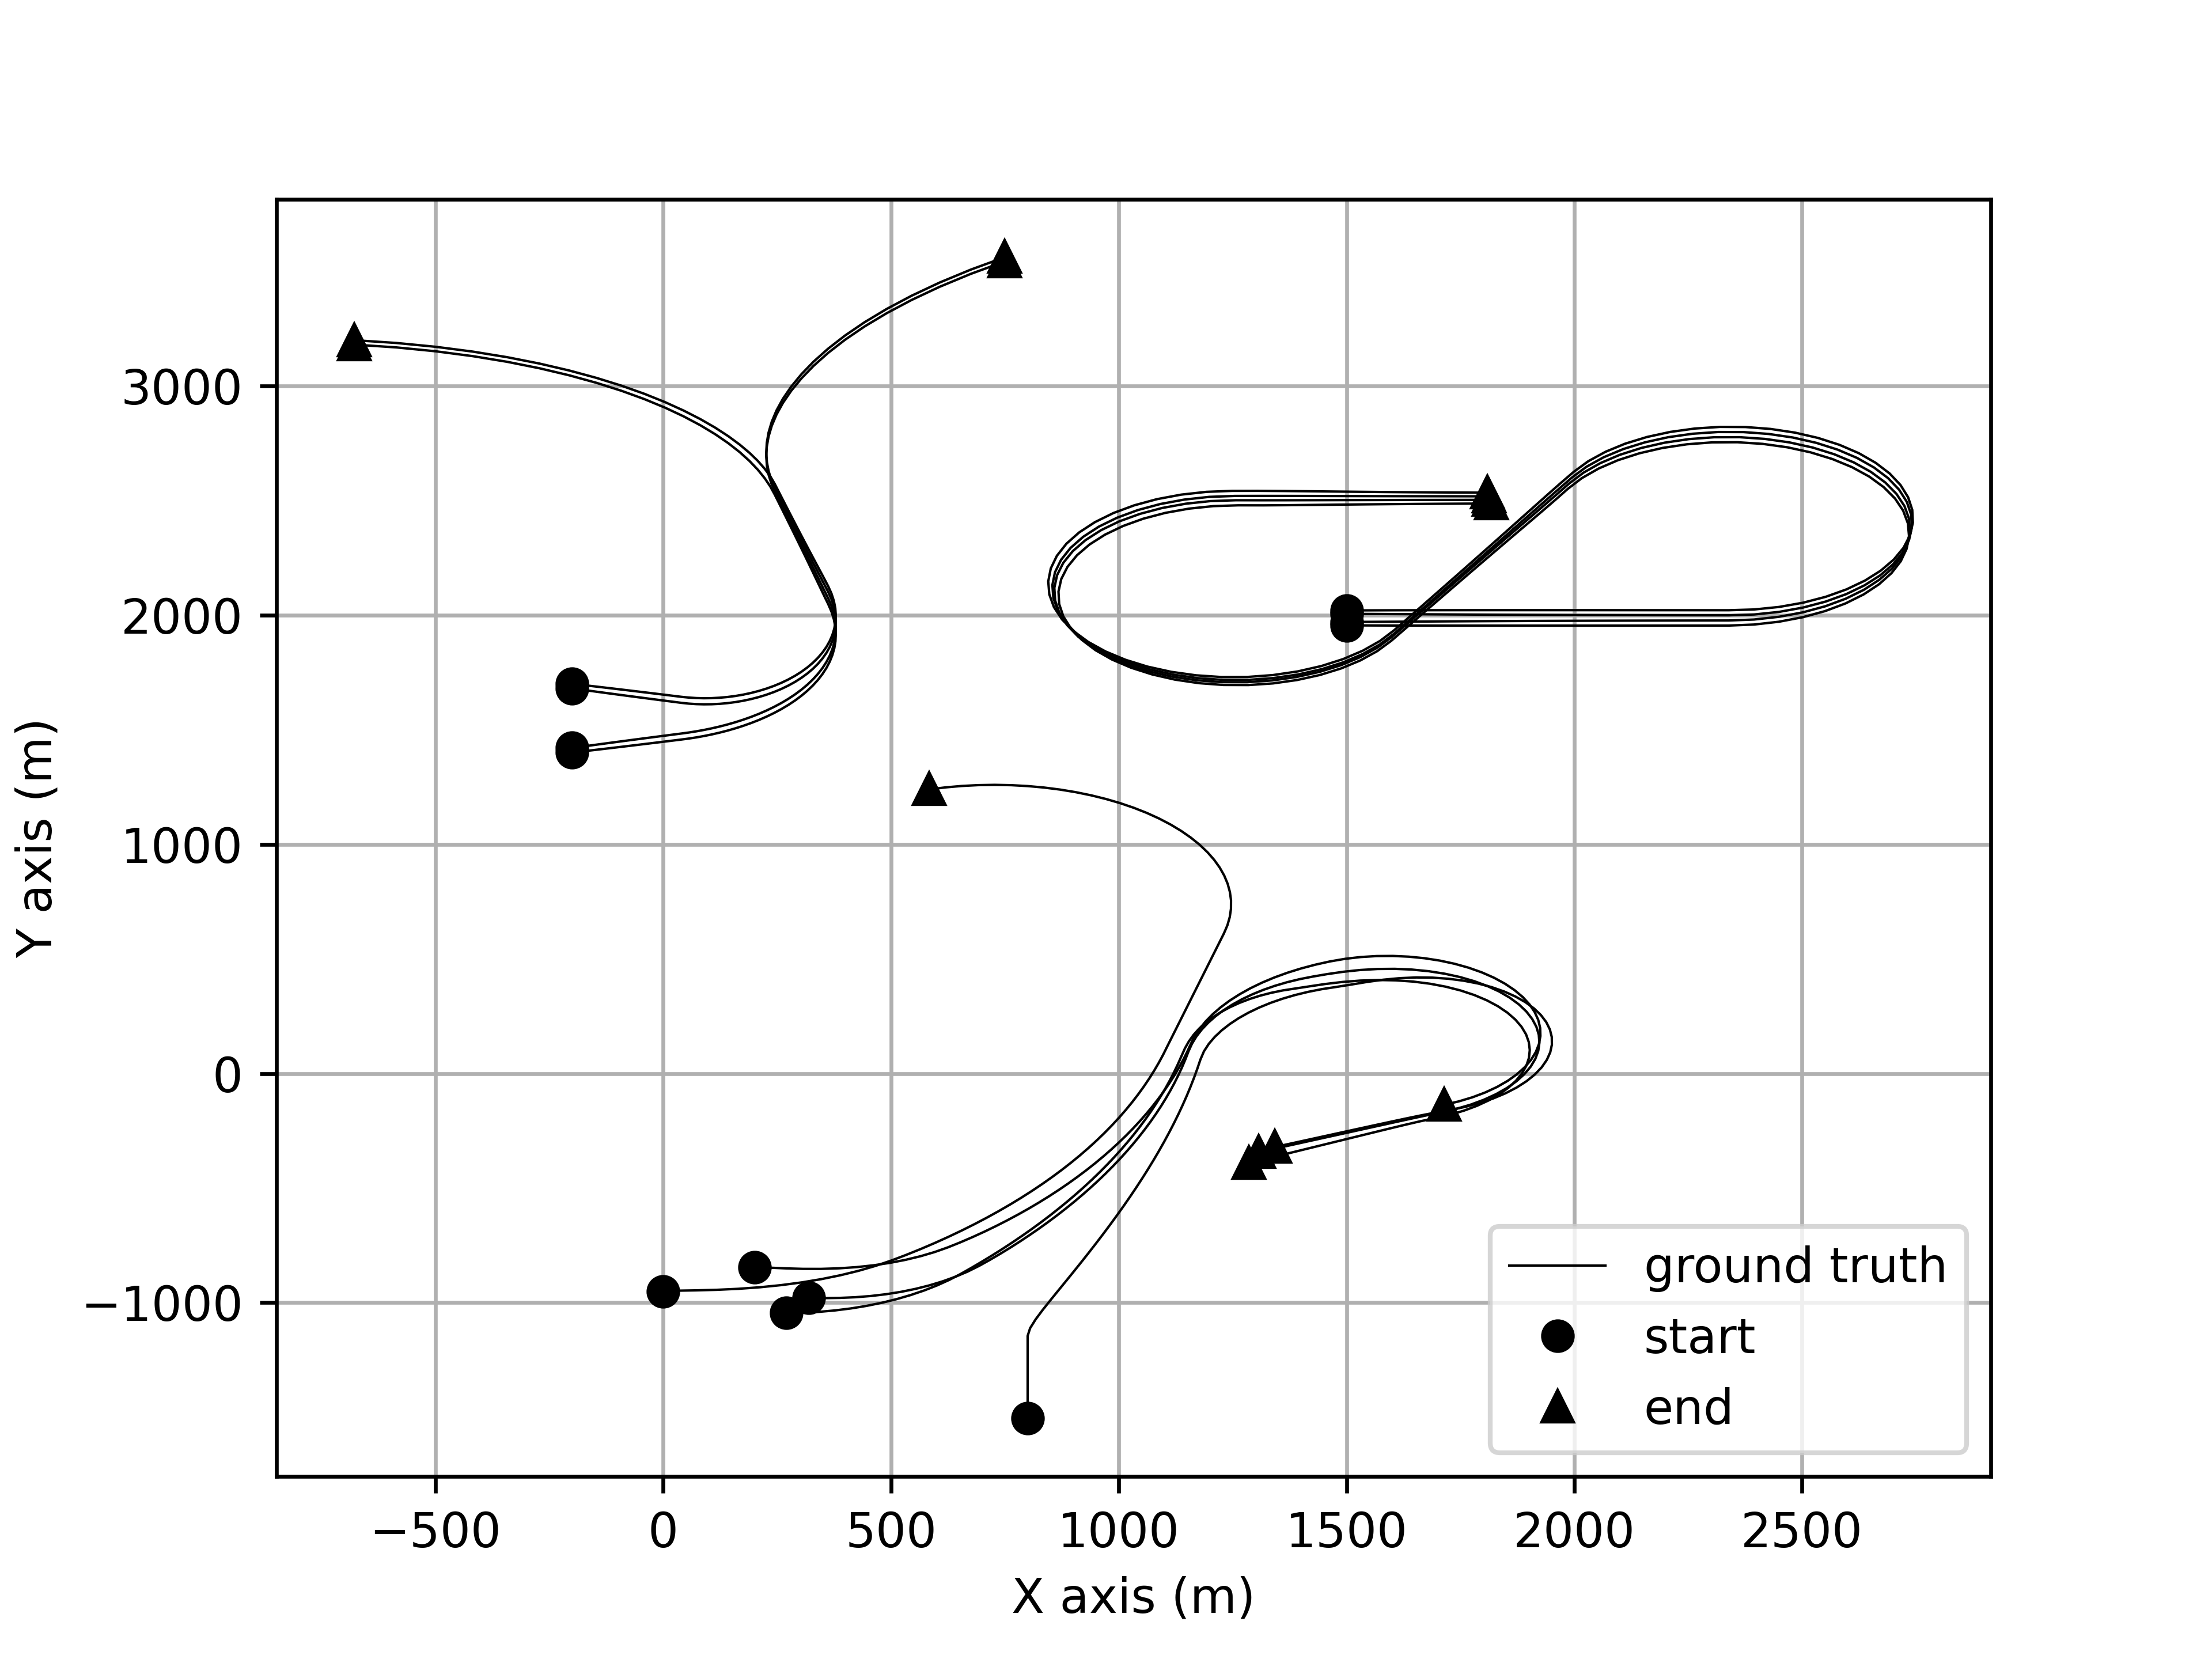
\includegraphics[width=0.78\linewidth]{figures/ground_truth.png}
\caption{The simulation scenario containing group merging, splitting, and coordinated maneuvers. The circle and triangle denote the starting and ending positions of each trajectory, respectively.}
\label{fig:simulation_scenario}
\end{figure}

Table~\ref{tab:simulation_scenario_ablation} presents the complete-tracker ablation under BP data association. P4 reduces the average OSPA error from 13.35 m for P2 to 12.85 m. P3 again differs little from the temporal model, whereas the peer-innovation variants improve both the matched position and velocity errors.

\begin{table}[!t]
\centering
\caption{Ablation results in the simulation scenario under the standard observation condition.}
\label{tab:simulation_scenario_ablation}
\resizebox{0.98\linewidth}{!}{
\begin{tabular}{c l c c c}
\hline
Index & Model & OSPA & Position(m) & Velocity(m/s) \\
\hline
P1 & Baseline &  &  & \\
P2 & Temporal & 13.35 & 6.33 & 3.82 \\
P3 & Own innovation & 13.34 & 6.32 & 3.80 \\
P4 & Full & \textbf{12.85} & \textbf{5.65} & \textbf{3.63}\\
\hline
\end{tabular}}
\end{table}

In the simulated scenario, three group target tracking methods are employed for comparison, and their performance is evaluated through Monte Carlo experiments. The evaluation metrics include the OSPA error and cardinality estimation. The compared methods are BP-R-RGTT \cite{li2024belief}, MCST-BP \cite{shen2024mcst}, and MTP-GO \cite{westny2023mtp}.
As shown in Fig. \ref{fig:trajectory1_OSPA_monte_carlo_multi_group}, the proposed SGGT-Net maintains consistently low OSPA errors throughout the tracking process. In contrast, the competing methods exhibit substantial error increases during maneuvering periods. Combined with the cardinality estimates in Fig. \ref{fig:trajectory1_Cardinality_monte_carlo_multi_group}, these methods suffer from repeated underestimation and overestimation of the target number, which partly accounts for the increased OSPA errors. By comparison, SGGT-Net provides more accurate and stable cardinality estimates throughout the scenario. 


\begin{figure}[!t]
	\centering
	\begin{minipage}[c]{0.9\linewidth}
		\centering
		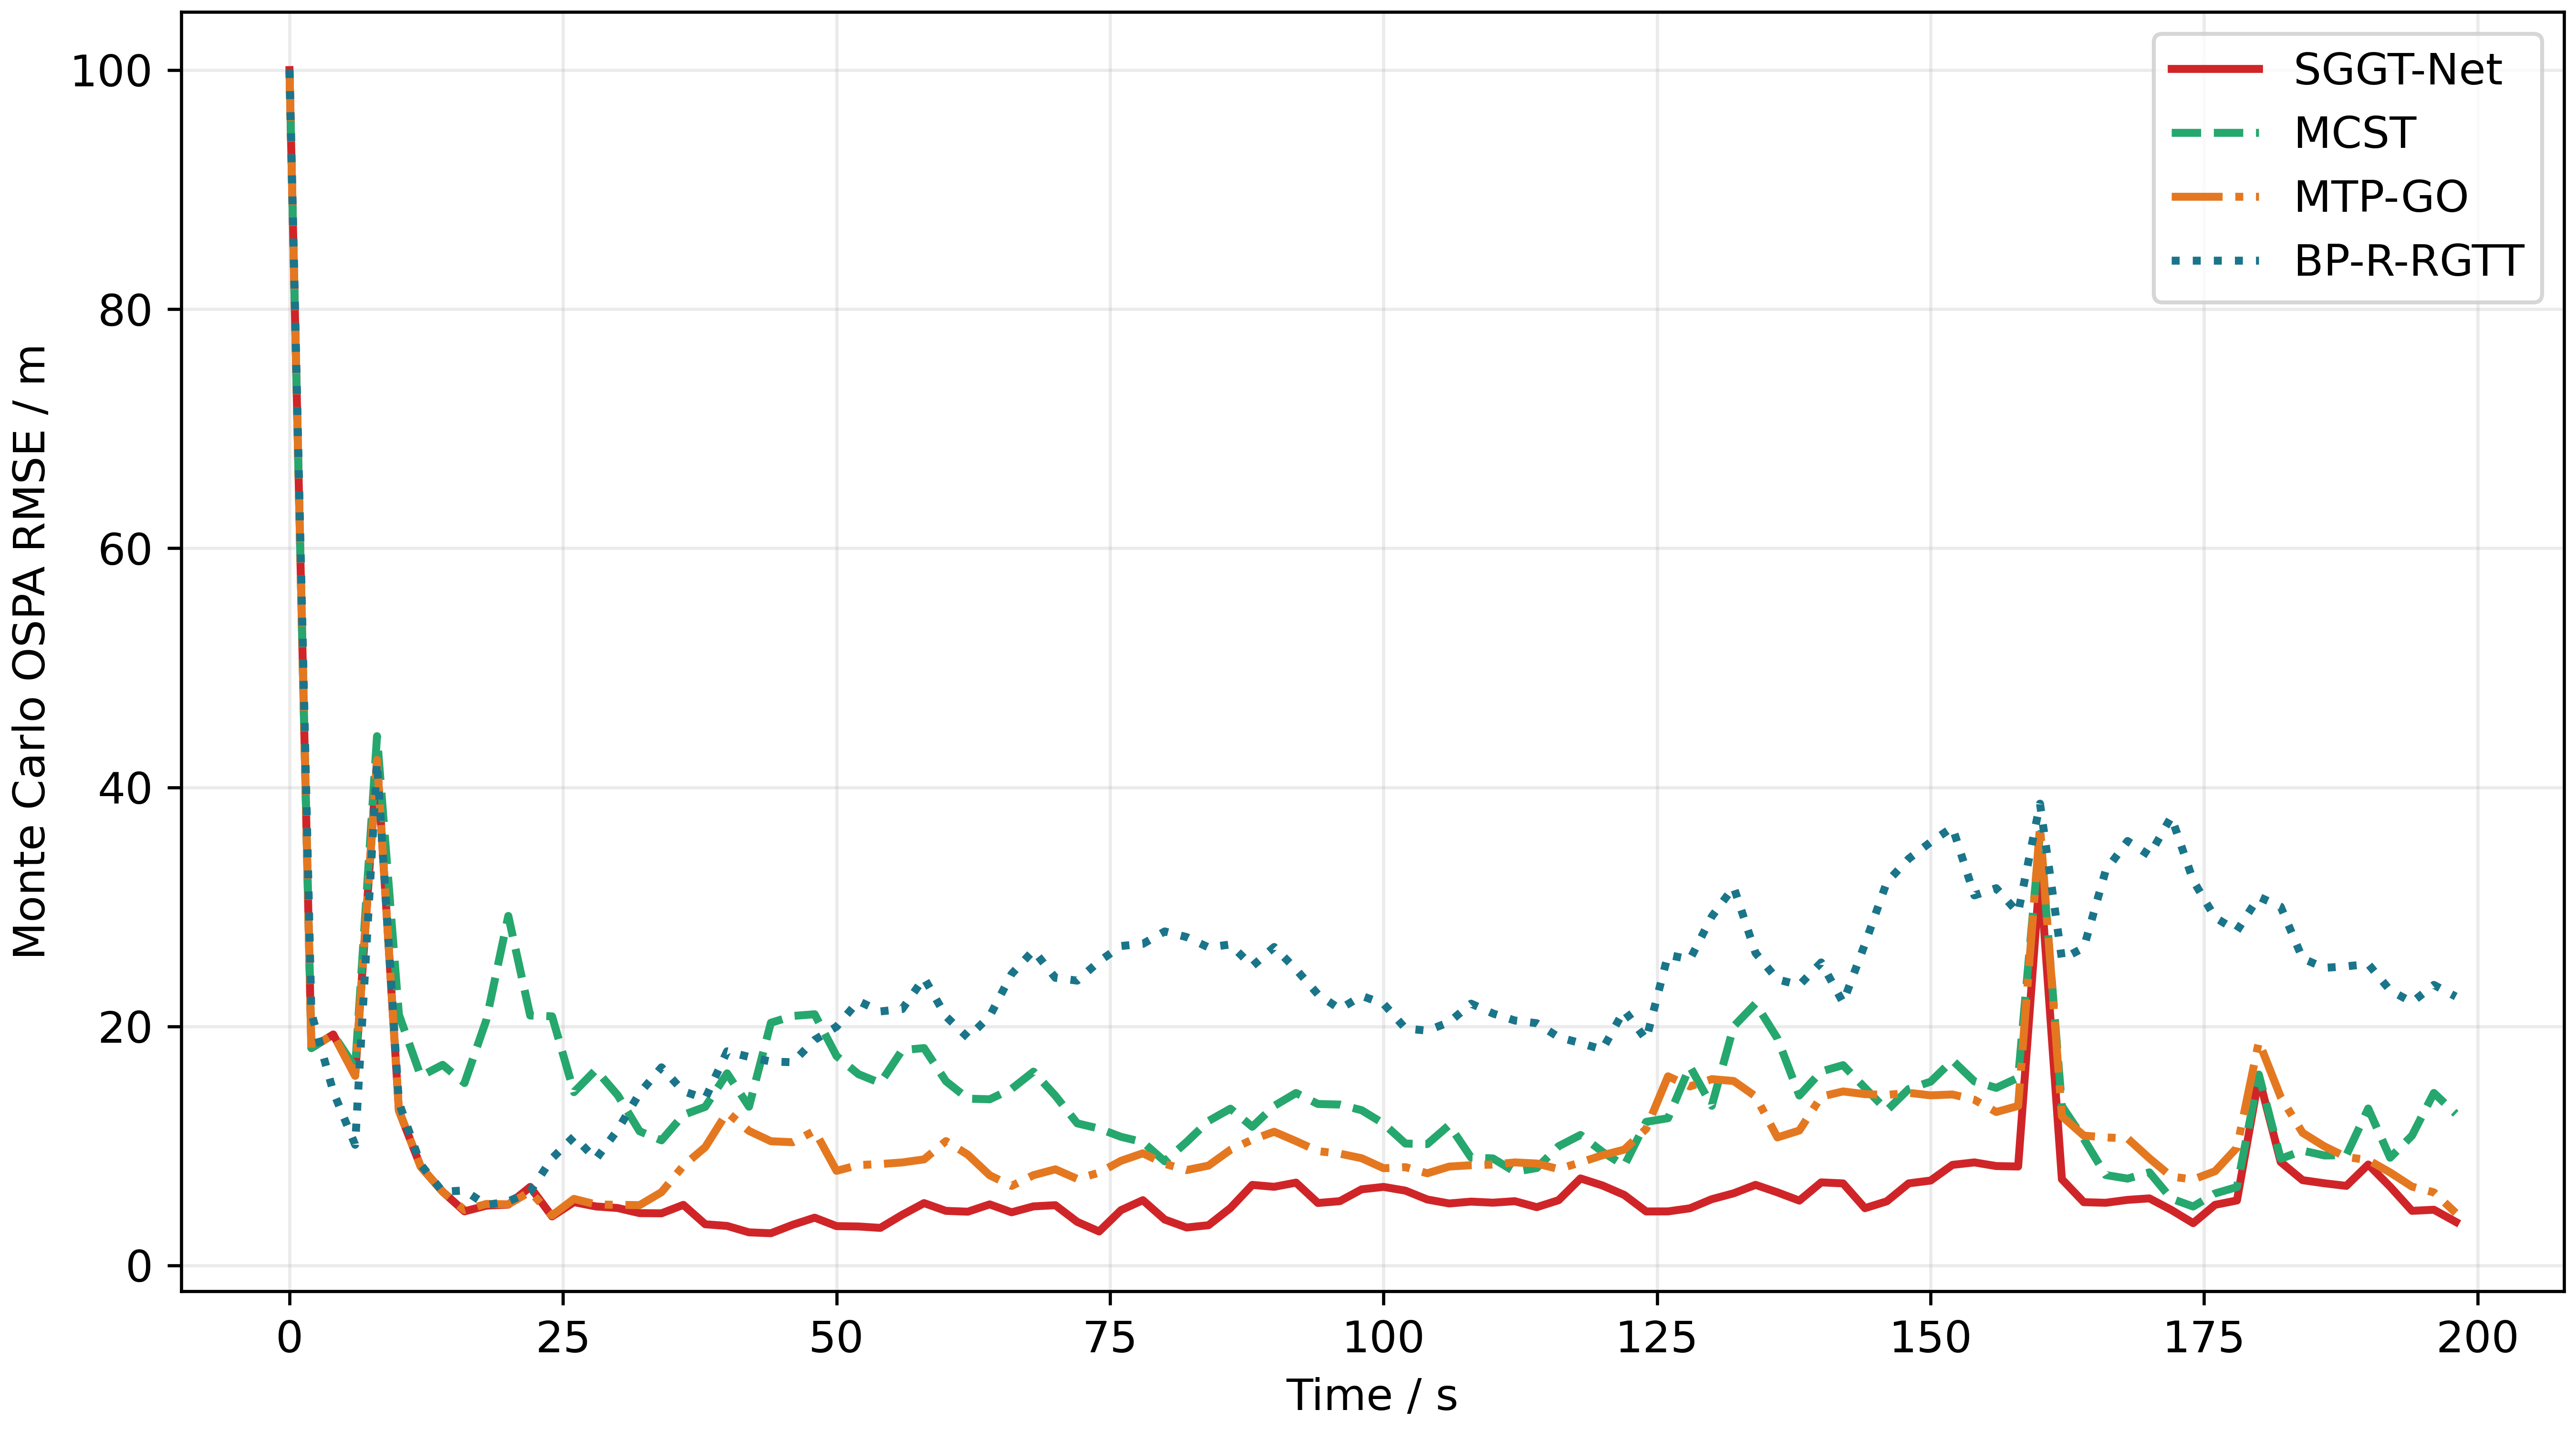
\includegraphics[width=1\linewidth]{figures/simulation_scenario_ospa_pd099_clutter3.png}
		\subcaption{}
		\label{fig:trajectory1_OSPA_monte_carlo_multi_group}%文中引用该图片代号
	\end{minipage}	
	\begin{minipage}[c]{0.9\linewidth}
		\centering
		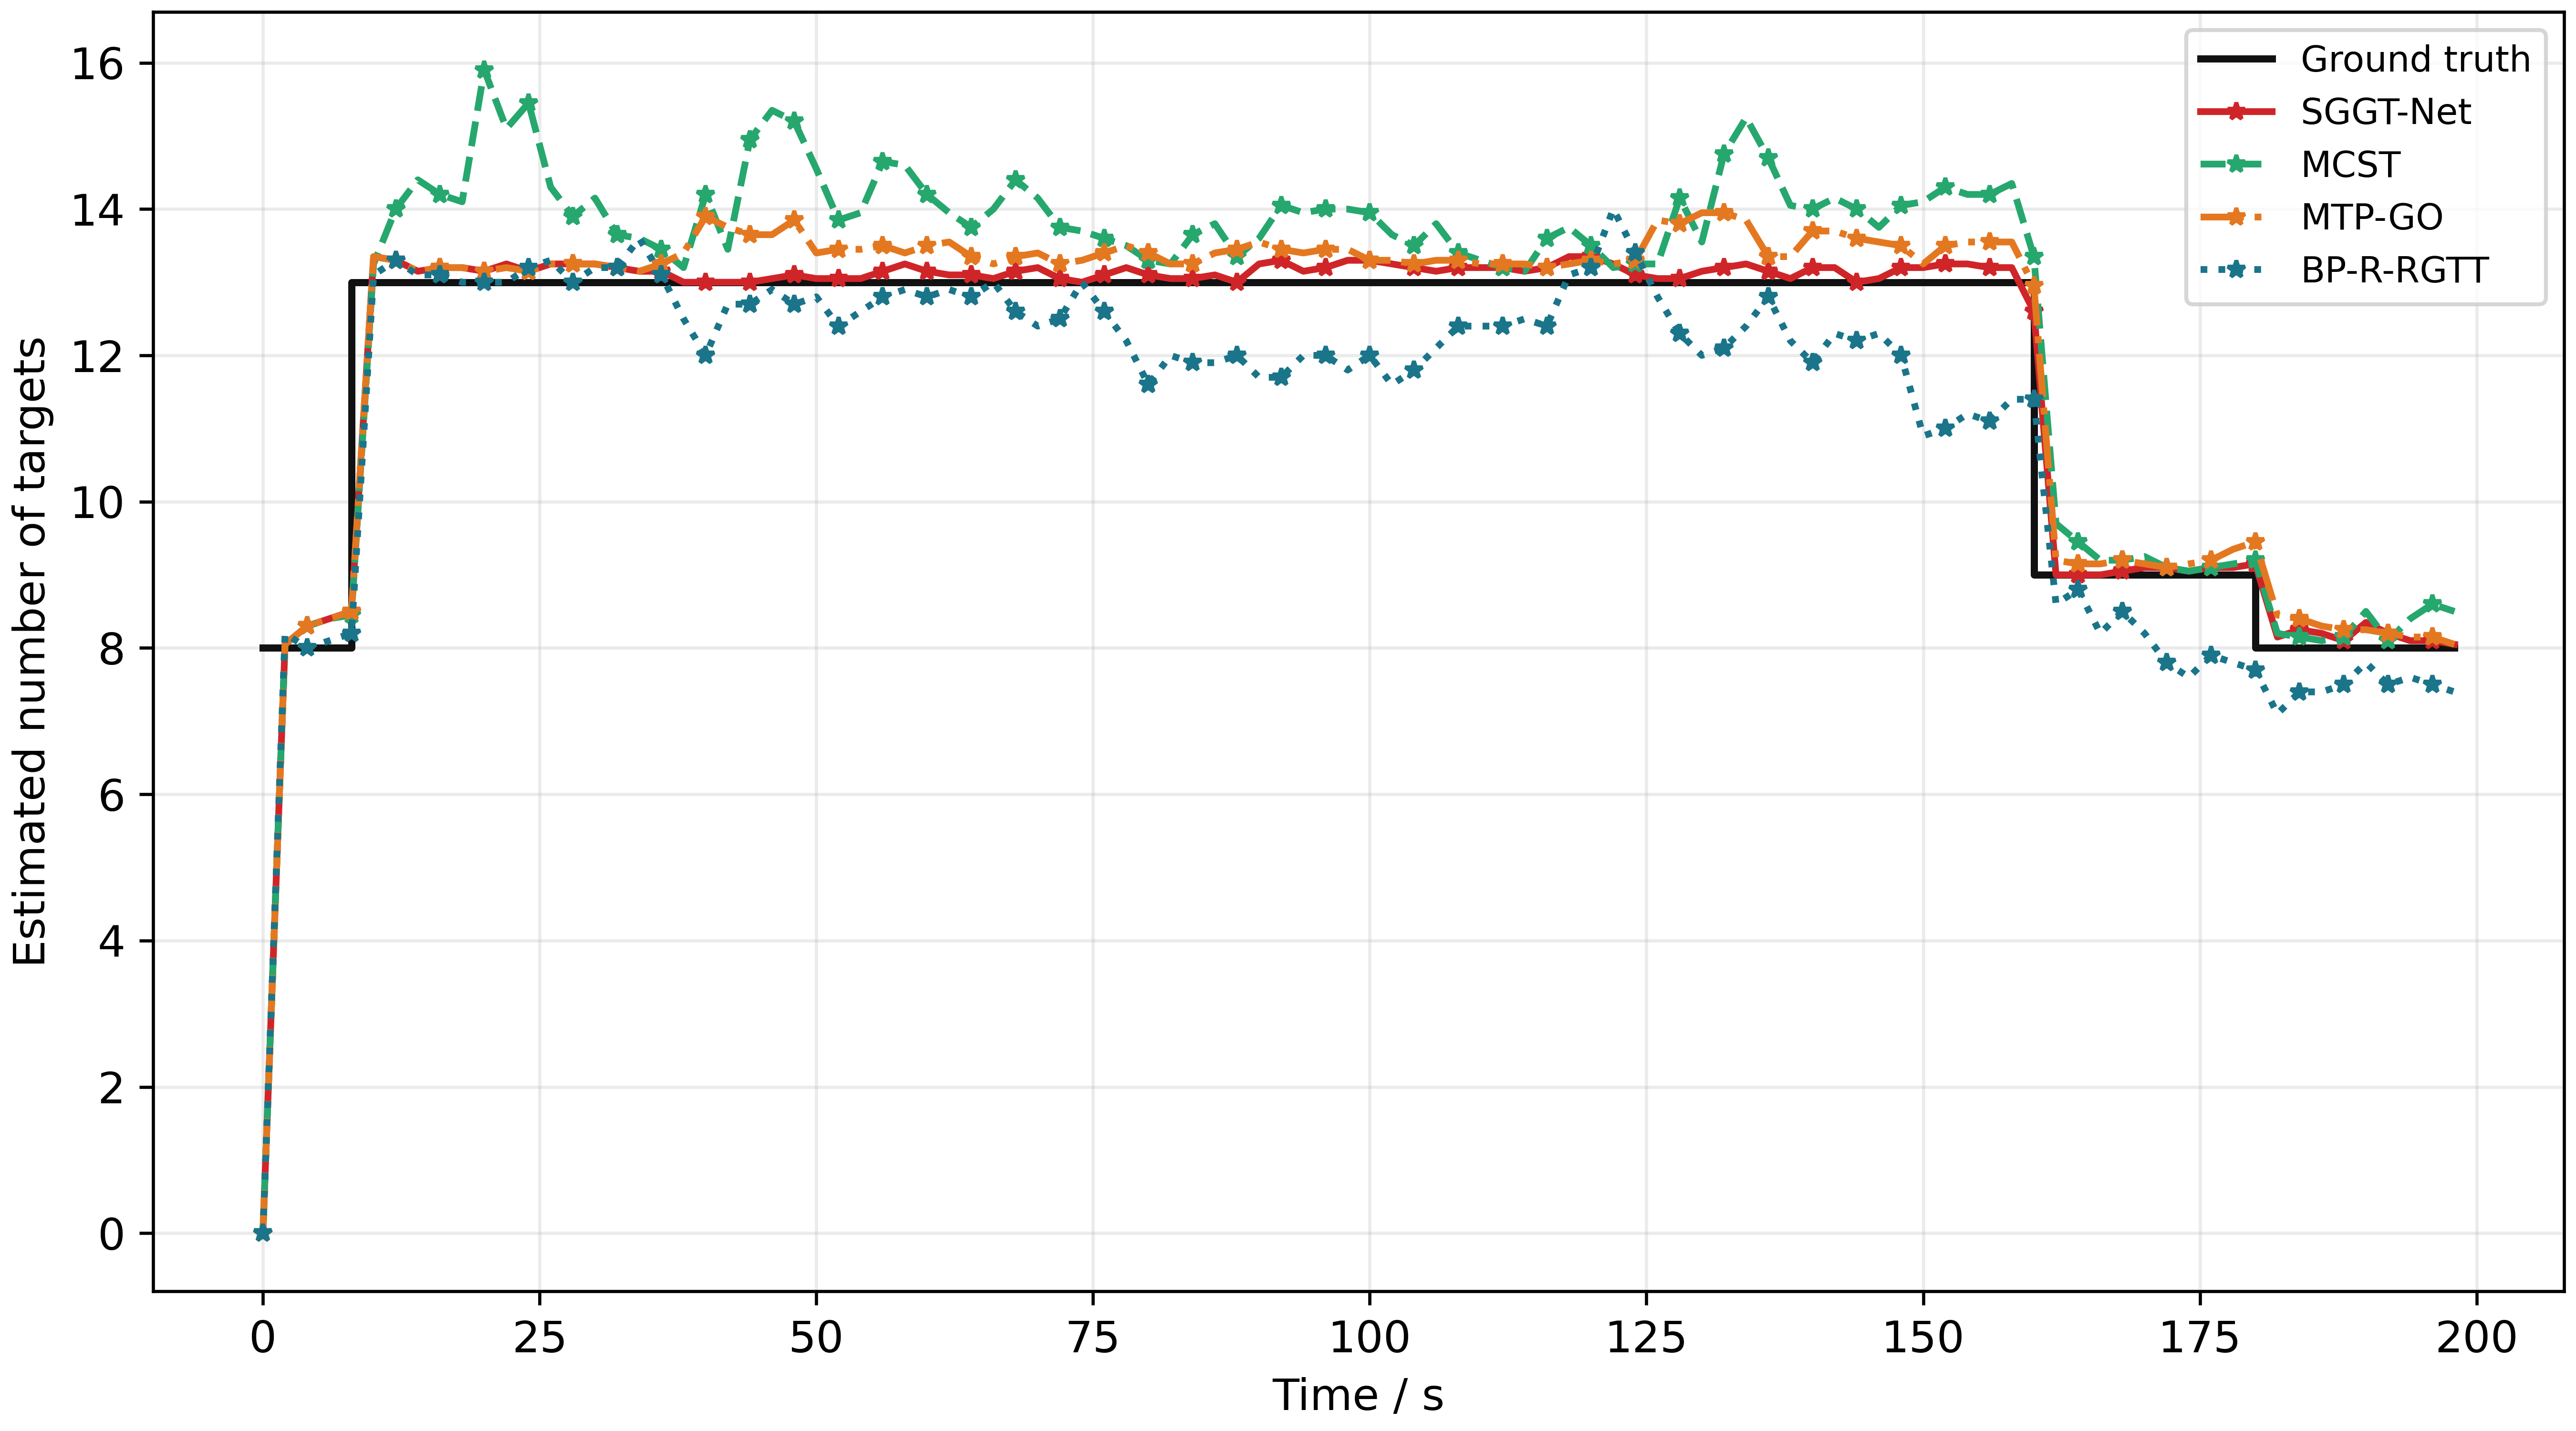
\includegraphics[width=1\linewidth]{figures/simulation_scenario_cardinality_pd099_clutter3.png}
		\subcaption{}
		\label{fig:trajectory1_Cardinality_monte_carlo_multi_group}%文中引用该图片代号
	\end{minipage}
	\caption{(a) OSPA error comparison: SGGT-Net vs. MCST-BP, MTP-GO, BP-R-RGTT (Complex Group Splitting/Merging). (b) Cardinality estimations comparison:  SGGT-Net vs. MCST-BP, MTP-GO, BP-R-RGTT (Complex Group Splitting/Merging).}
	\label{fig:simulation_scenario_comparison}%文中引用该图片代号
\end{figure}


\subsubsection{Robustness Analysis}
To evaluate the robustness of the proposed method under different environments, we conducted experiments under various detection probabilities and clutter densities, respectively.
\begin{enumerate}
	\item  Varying detection probability \(P_{d}\): Table \ref{tabel:pos_est_monte_carlo_pd} shows the average OSPA errors of all algorithms under different detection probabilities. When target misdetection occurs, the tracking performance entirely relies on model prediction. The results demonstrate that SGGT-Net still achieves lower OSPA errors even under low detection probabilities, which benefits from the accurate modeling of group target kinematics by the network.
	
	\item Varying clutter density \(\mu_{c}\): The mean OSPA errors of each algorithm under diverse clutter densities are detailed in Table \ref{tabel:pos_est_monte_carlo_mu_c}. As expected, the tracking performance of all algorithms degrades as the clutter density increases, mainly due to the increased uncertainty in the data association process. Overall, the proposed SGGT-Net maintains stable tracking performance in heavy clutter environments.
\end{enumerate}

\begin{table}[h!]
	\centering
	\caption{OSPA errors (m) of all algorithms vs. different \(P_{d}\).}
	\label{tabel:pos_est_monte_carlo_pd}
	\normalsize
	\resizebox{0.8\linewidth}{!}{
		\begin{tabular}{ c c c c c }	
			\hline 
			&   SGGT-Net& MCST-BP & MTP-GO & BP-R-RGTT\\
			\hline
			\(P_{d} = 0.95\)&  12.85& 22.64 & 15.39 & 25.33 \\
			\(P_{d} = 0.85\)& 17.70 & 27.95  & 20.98  & 29.15   \\
			\(P_{d} = 0.75\)& 23.48  & 31.40  & 27.54  &  33.94  \\
			\hline
		\end{tabular}
	}
\end{table}	

\begin{table}[h!]
	\centering
	\caption{OSPA errors (m) of all algorithms vs. different \(\mu_{c}\).}
	\label{tabel:pos_est_monte_carlo_mu_c}
	\normalsize
	\resizebox{0.8\linewidth}{!}{
		\begin{tabular}{ c c c c c }	
			\hline 
			&   SGGT-Net& MCST-BP & MTP-GO & BP-R-RGTT\\
			\hline
			\(\mu_{c} = 10\)&  12.85& 22.64 & 15.39 & 25.33 \\
			\(\mu_{c} = 20\)& 18.28  & 28.61  & 22.61  & 29.65   \\
			\(\mu_{c} = 30\)& 24.54  & 36.90  & 27.14  &  35.90  \\
			\hline
		\end{tabular}
	}
\end{table}	


\subsection{Computational Complexity Analysis}

Table \ref{tab:complexity} reports the measured neural network inference time and peak memory usage for different numbers of targets. Within the evaluated range, the inference time varies only marginally with the target number. P4 requires approximately 2--3 ms more computation per frame than P2. The innovation histories are maintained in a shared slot-indexed buffer, and peer information is obtained through sparse aggregation. Consequently, the complete model requires only approximately 0.07 MiB more peak allocated CUDA memory than the temporal baseline over the evaluated target-number range.

Table \ref{tabel:time_monte_carlo_multi_groups} reports the average processing time per frame of all compared methods under \(P_d=0.95\) and \(\mu_c=10\). MTP-GO also employs a graph neural network-based encoder and a Neural ODE-based decoder. In comparison, SGGT-Net introduces additional computation for spectral graph processing and neural dynamics prediction, resulting in slightly higher computational complexity than MTP-GO. Nevertheless, its average processing time remains acceptable for real-time or near-real-time applications.

Overall, these results demonstrate that SGGT-Net achieves a favorable trade-off between tracking accuracy and computational efficiency, supporting its practical deployment in complex multi-target tracking scenarios.


\begin{table}[!t]
\centering
\caption{Neural motion-predictor complexity versus target number.}
\label{tab:complexity}
\resizebox{0.96\linewidth}{!}{
\begin{tabular}{c cc cc}
\hline
Targets & P2 time (ms) & P4 time (ms) & P2 memory (MiB) & P4 memory (MiB)\\
\hline
5  & 98.14 & 101.55 & 10.62 & 10.69\\
10 & 99.82 & 101.47 & 10.68 & 10.79\\
20 & 100.31 & 102.80 & 10.81 & 10.87\\
40 & 100.53 & 102.79 & 11.07 & 11.14\\
\hline
\end{tabular}}
\end{table}


\begin{table}[h!]
	\centering
	\caption{Execution time (ms/frame) of all algorithms with complex group splitting and merging.}
	\label{tabel:time_monte_carlo_multi_groups}
	\normalsize
	\resizebox{0.9\linewidth}{!}{
		\begin{tabular}{c c c c c }	
			\hline 
			& MCST-BP& MTP-GO & BP-R-RGTT & SGGT-Net\\
			\hline
			Time (ms) & 342.80 & 82.13 & 184.70 & 101.96\\
			\hline
		\end{tabular}
	}
\end{table}
 

\section{Conclusion}

This paper presents SGGT-Net for motion prediction and recursive state estimation of maneuvering group targets in cluttered environments. A streaming graph
temporal encoder and a Neural ODE decoder are employed to generate a one-step basic motion prior. Historical residuals are processed by a smooth temporal
spectral filter to extract persistent prediction mismatch. A causal group-innovation corrector then represents the target innovation and the leave-one-out
peer innovation through separate branches. The raw and whitened innovations, normalized innovation magnitude, and innovation-covariance descriptors provide
complementary motion information using only data available before the predicted time step. 

SGGT-Net is incorporated into a BP tracking framework through marginal association probabilities and a moment-matched measurement update. The independent
trajectory experiments show that the peer-innovation branch improves prior position prediction, with larger gains during motion switches, strong maneuvers,
and OOD motion. In complete BP tracking, the resulting model reduces the OSPA error relative to the temporal predictor under the standard simulation
condition. In the experiments to verify the robustness, the proposed model also demonstrated the highest estimation accuracy. The shared innovation buffer and sparse peer aggregation also keep the additional peak allocated CUDA memory close to that of the
temporal model. Future work will focus on extending the framework to multi-sensor settings and improving computational efficiency for real-time applications.

\bibliographystyle{IEEEtaes}
\bibliography{ref}

\begin{IEEEbiography}
[{
\includegraphics[width=1in,height=1.25in,clip,keepaspectratio]{figures/skl.jpg}}]
{Kailun Shen} was born in Jiangsu, China, in 1999. He is currently working toward the Ph.D. degree with the Institute of Information Sensing, Xidian University, Xi'an, China. His main research interests include target detection and target tracking.
\end{IEEEbiography}

\begin{IEEEbiography}
[{
\includegraphics[width=1in,height=1.25in,clip,keepaspectratio]{figures/ywm.png}}]
{Weiming Yuan} was born in Shandong Province, China, in 1976. He received the B.S. degree in electronic engineering and the Ph.D. degree in information and communication engineering from Xidian University, Xi'an, China, in 1999 and 2005, respectively. He is currently a Professor with the Institute of Information Sensing, Xidian University. His main research interests include signal processing and data processing.
\end{IEEEbiography}

\end{document}
